\documentclass{article}
\usepackage
[
        a4paper,% other options: a3paper, a5paper, etc
        left=2.5cm,
        right=2.5cm,
        top=3cm,
        bottom=3cm,
        % use vmargin=2cm to make vertical margins equal to 2cm.
        % use hmargin=3cm to make horizontal margins equal to 3cm.
        % use margin=3cm to make all margins  equal to 3cm.
]
{geometry}
%\usepackage[utf8]{inputenc}
%\usepackage{amssymb}
%\usepackage{graphicx}
\usepackage{hyperref}
%\usepackage[demo]{graphicx}
\usepackage{graphicx}
\usepackage{subcaption}
\usepackage[ruled,linesnumbered]{algorithm2e}
\usepackage{amsmath}
\usepackage{lscape}
\usepackage{fancyhdr}
\usepackage{tikz-network}
\usepackage{cite}
\usepackage{xepersian}
\captionsetup[subfigure]{justification=justified,singlelinecheck=false}

\settextfont[Scale=1.25]{XBNiloofar.ttf}
\setlatintextfont[Scale=1.2]{Times New Roman}
\setdigitfont[Scale=1.25]{XBNiloofar.ttf}
\renewcommand{\baselinestretch}{1.5}
\graphicspath{{fig/}}  

%%%%%%%%%%%%%%%%%%%%%%%%%%%%%%%%%% header
\pagestyle{fancy}
\fancyhf{}
\rhead{سعید تقوی / اثر تحریک مغز بر فعالیت نوسانی شبکه های مغز}
\lhead{\thepage}
%%%%%%%%%%%%%%%%%%%%%%%%%%%%%%%%%% end header


%%%%%%%%%%%%%%%%%%%%%%%%%%%%%%%%%% title, author

\title{اثر تحریک مغز بر فعالیت نوسانی شبکه های مغز}
\author{سعید تقوی
\LTRfootnote{Email: s.taghavi@iasbs.ac.ir} 
\\
استاد راهنما: علیرضا ولیزاده
\LTRfootnote{Email: valizadeh@iasbs.ac.ir} 
 \\
{\small 
 دانشكدهٔ فیزیک، دانشگاه تحصیلات تكمیلی علوم پایهٔ زنجان، صندوق پستی 45195-1159، زنجان، ایران
 }
 \\
} 
% \date{\today}
%%%%%%%%%%%%%%%%%%%%%%%%%%%%%%%%%% end title, author


\begin{document}
\maketitle
\setcounter{page}{1}

%%%%%%%%%%%%%%%%%%%%%%%%%%%%%%%%%% abstract
\begin{abstract}
طی سه دهه اخیر مطالعات و آزمایشات گسترده انجام شده نشان داده‌اند که ریتم‌های مغزی و نوسانات گروهی سلول‌های عصبی نقشی بنیادی در کنترل تبادل اطلاعات بین نواحی مختلف مغز و در نتیجه در پردازش اطلاعات و شکل‌دهی کارکردهای شناختی مختلف از جمله ادراک حسی، توجه، حافظه، و آگاهی ایفا می‌کنند. اختلال در الگوی نوسانی نواحی مختلف مغز در بسیاری از بیماری‌های سیستم عصبی مشاهده و ثبت شده است. امروزه شواهد محکمی وجود دارند که اختلال در الگوی نوسانات مغزی، نه تنها یک نشانه بلکه دلیل بوجود آمدن ناهنجاری‌های شناختی و عصبی است. بنابر این شواهد، بازتولید الگوی نوسانی مغز سالم در درمان‌های مختلف موجب بهبود نشانه‌های بیماری می‌شود و تحقق آن به کمک روش‌های درمانی مختلف از جمله درمان‌های دارویی، بازتوانی شناختی و تحریک مغزی از جمله معیارهای مورد نظر پژوهشگران است. 

تحریک مغزی یکی از روش‌های درمانی است که همزمان با درمان دارویی و یا در مواردی که مداخلات دارویی پاسخ مناسبی نمی‌دهد، استفاده شده و کارآیی آن در طیف وسیعی از بیماری‌های شناختی و عصبی مشاهده شده‌ است. با این حال سازوکار تاثیر آن بر شبکه‌های عصبی و علت کارایی آن در بسیاری از موارد ناشناخته است و کاربرد و توسعه آن بر اساس تجربیات مستند شده یا آزمون و خطا انجام می‌گیرد.

برای تحلیل نوع تاثیر تحریک مغزی بر فعالیت جمعی نورون‌ها، شناخت مواردی چون اصول حاکم بر دینامیک فعالیت شبکه‌های عصبی، خواص الکتریکی نورون‌ها، خواص فیزیکی و ساختار شبکه مورد تحریک  لازم است. درک صحیح نظری از رفتار دینامیکی جمعیت‌های نورونی تحت تاثیر تحریک می‌تواند به بهبود روش‌های تحریک کمک کند و همچنین پیش‌بینی اثر تحریک بر روی عملکرد مغز را امکان‌پذیر نماید. در پژوهش پیش رو اثر تحریک بر فعالیت نوسانی جمعی نورون‌ها و اثر آن در بیماری‌ها و ناهنجاری‌های مختلف بررسی خواهد شد.

کلمات کلیدی: 
همگامی سیستم عصبی، تحریک مغز، نوسانات عصبی

\newpage


\end{abstract}
% \pagebreak
%%%%%%%%%%%%%%%%%%%%%%%%%%%%%%%%%% end abstract


%\begin{document}

\flushbottom % Makes all text pages the same height

\tableofcontents % Print the contents section

\thispagestyle{empty} % Removes page numbering from the first page

%----------------------------------------------------------------------------------------
%	ARTICLE CONTENTS
%----------------------------------------------------------------------------------------
\section{مقدمه}

فرآیندهای همگام سازی در سیستم عصبی نقش مهمی دارند؛ به عنوان مثال، در زمینه پردازش اطلاعات و کنترل حرکتی. 
با این حال، همگامیِ بیش از حدِ طبیعی و کمتر از حدِ طبیعی باعث بروز اختلال در الگوی فعالیت نوسانی نواحی مختلف مغز می‌شود و عملکرد مغز را به شدت مختل می‌کند و مشخصه بسیاری از بیماری‌ها و اختلالات عصبی می‌باشد.
%با این حال، همگامی بیش از حد ممکن است عملکرد مغز را به شدت مختل کند و مشخصه بسیاری از اختلالات عصبی همین همگامی بیش از حد و ناهنجار است.
اختلالات عصبی متعددی، مانند پارکینسون، لرزش اساسی
\LTRfootnote{Essential Tremor (ET)}
 ، وزوز گوش
\LTRfootnote{Tinnitus}
و صرع با همگامی قوی و غیرعادی فعالیت نورون‌ها مشخص می‌شوند. کاهش نوسانات همگامِ غیرعادی در این بیماران با بهبود علائم بیماری همراه است 
\cite{uhlhaas2006neural}.
%برای مثال کاهش نوسانات باند بتا به کمک داروها دوپامینرژیک یا تحریک عمیق مغز با فرکانس بالا با بهبود علائم حرکتی در بیماران پارکینسونی ارتباط مثبت دارد. 
%اختلالات مغزی متعددی مانند بیماری پارکینسون، لرزش اساسی، صرع و وِزوِز گوش با همگامی غیر طبیعی نورون ها همراه هستند.
برای نمونه، در پارکینسون همگامی بیش از حد در ناحیه بیزل گانگلیا\LTRfootnote{Basal ganglia}
  با اختلالات حرکتی همراه است
 \cite{hammond2007pathological}
 ، در حالی که نورون‌ها در شرایط فیزیولوژیکی عادی به دور از همگامی کامل آتش می‌کنند.  کاهش نوسانات همگام در فرکانس‌های باند بتا (از ۸ تا ۳۵ هرتز) به کمک داروهای دوپامینرژیک با بهبود علائم حرکتی در بیماران پارکینسونی همبستگی مثبت دارد
  \cite{hammond2007pathological, kuhn2006reduction}.
  از طرف دیگر، تحریک هسته ساب تالامیک
\LTRfootnote{Subthalamic nucleus (STN)}
با فرکانس پایین (۵ تا ۲۰ هرتز)، که برای تقویت نوسانات همگام در همین فرکانس‌ها در نظر گرفته شده است منجر به وخامت بالینی قابل توجهی در علائم پارکینسون و عملکردهای حرکتی در انسان‌های بیمار و جوندگان پارکینسونی می‌شود
\cite{jenkinson2011new, moro2002impact, timmermann2004ten, eusebio2008effects, barnikol2008tremor, chen2011stimulation}.
در اختلال وزوز گوش نیز الگوهای غیر طبیعی افزایش فعالیت عصبی همگام در بیماران انسانی و مدل های جانوری مشاهده شده است
\cite{weisz2005tinnitus, weisz2007neural, dohrmann2007tuning, adamchic2014reversing}.
 به طور خاص، ریتم های عصبی پاتولوژیک بالا و مداوم در باند دلتا (۱/۵ تا ۴ هرتز) همچنین در فرکانس های باند گاما (بیشتر از ۳۰ هرتز) در بیماران مبتلا به وزوز گوش مزمن در مقایسه با افراد سالم دیده شد که با پریشانی مرتبط با وزوز گوش و بلندی وزوز گوش همبستگی دارد
 \cite{weisz2005tinnitus, weisz2007neural, lorenz2009loss}.
  علاوه بر این، یک ارتباط مثبت بین هنجارسازی این فعالیت‌های نورونی و کاهش شدت وزوز گوش وجود دارد
\cite{weisz2005tinnitus, weisz2007neural, dohrmann2007tuning, adamchic2014reversing, lorenz2009loss}.  
 در شکل
\ref{fig:et-time-freq-analysis}
نیز می‌توان افزایش توان نوسانات مغزی یک بیمار مبتلا به لرزش اساسی را در محدوده فرکانسی ۱۰ هرتز مشاهده کرد.
\begin{figure}[t!]
     \centering
     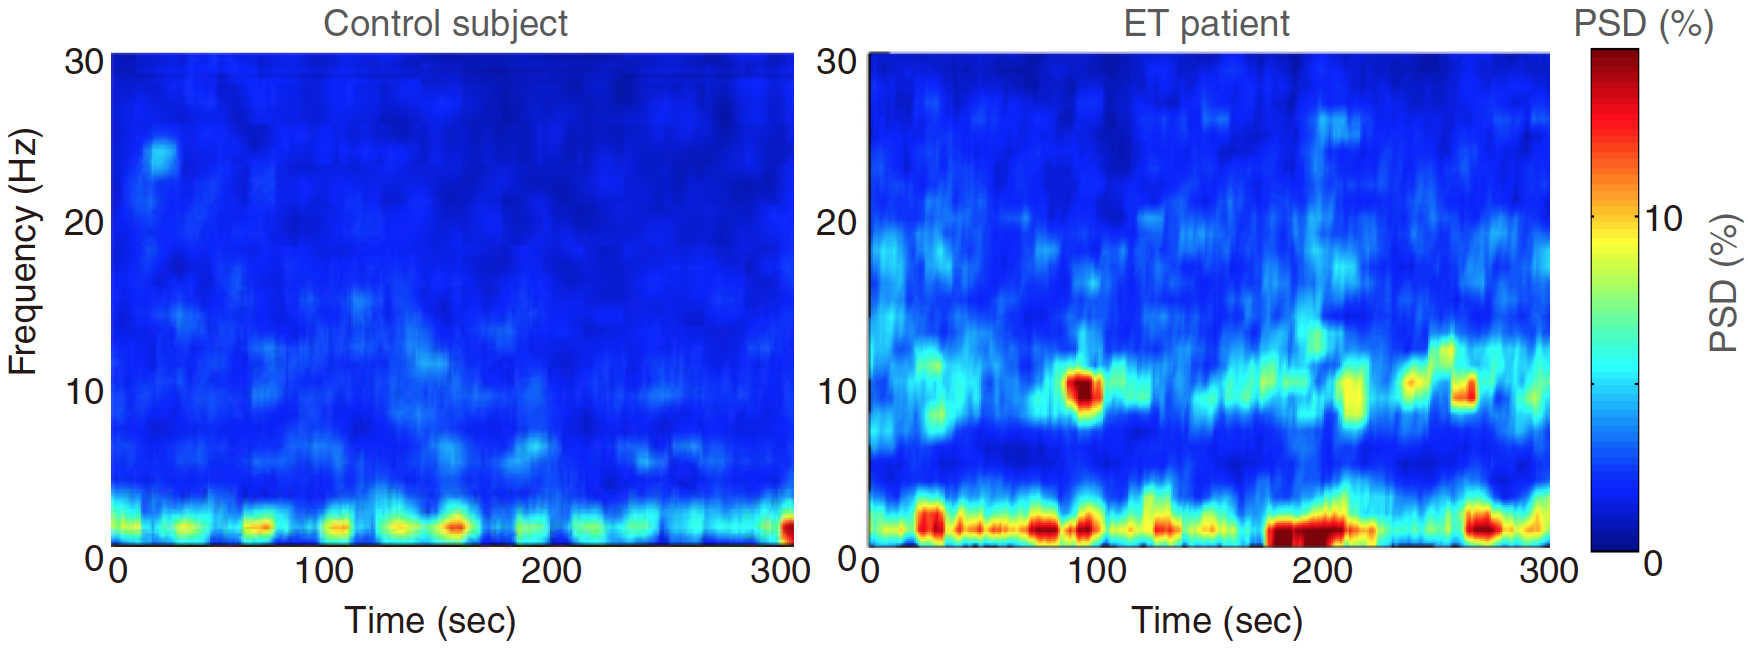
\includegraphics[width=0.9\textwidth]{et}
     \caption{مقایسه تحلیل فرکانسی نوسانات مغزی بیمار مبتلا به لرزش اساسی و نمونه کنترل }
     \label{fig:et-time-freq-analysis}
\end{figure}
   روی هم رفته، همگامی غیر عادی فعالیت نورون‌ها می‌تواند به طور قابل توجهی فرآیندهای عصبی و عملکردهای مغزی را مختل کند و به عنوان یک هدف برای درمان های جدید بکار می‌رود.


امروزه درمان استاندارد برای بیماران پارکینسون مقاوم به درمان دارویی، تحریک عمیق مغز با فرکانس بالا
\LTRfootnote{High-frequency deep brain stimulation (HF-DBS)}
است. برای این منظور یک قطار پالس فرکانس بالا (بیشتر از ۱۰۰ هرتز) از طریق الکترودهایی که در عمق مغز کاشته شده است به قسمت‌های مشخصی از مغز اعمال می‌شود. درمان بیماری‌های عصبی و روانی شدید مانند پارکینسون، لرزش، درد خیالی و مزمن
\LTRfootnote{Chronic and phantom pain}
\footnote{درد فانتوم دردی است که در فقدان یک عضو از بدن درک می‌شود. فقدان عضو می‌تواند در نتیجه قطع عضو یا فقدان مادرزادی عضو باشد.}
، افسردگی اساسی
\LTRfootnote{Major depression disorder (MDD)}
، وسواس فکری و عملی
\LTRfootnote{Obsessive–compulsive disorder (OCD) }
%، سندروم توره
%\LTRfootnote{Tourette syndrome}
 و صرع به کمک تحریک عمیق مغز یک زمینه در حال رشد و امیدوار کننده است. با اینکه تا کنون مکانیزم‌های اثر تحریک عمیق مغز با فرکانس بالا کاملا شناخته نشده‌اند؛
%  چند مکانیزم دخیل در نتایج مشاهده شده
%%  از تحریک عمیق مغز با فرکانس بالا 
%  ممکن است مکانیزم مسدود کردن
%\LTRfootnote{Jamming}
%، مهار غشا، تحریک نورون‌های تحریکی و مهاری آوران
%\LTRfootnote{Afferent}
%، تحریک نورون‌های وابران
%\LTRfootnote{Efferent}
%، شکل پذیری دستگاه عصبی باشند
%\cite{benabid2005putative}.
مهمترین گزینه‌های نحوه اثر گذاری آن مکانیزم مسدود کردن
\LTRfootnote{Jamming}
و همچنین شکل پذیری دستگاه عصبی می‌باشد
\cite{benabid2005putative}.
%از نوشته دکتر ولیزاده برای طرح پژوهشی بنیاد نخبگان:

استفاده از مدل‌های محاسباتی برای شبیه‌سازی سلول‌های عصبی ناحیه‌ای از مغز 
%و برهمکنش آن‌ سلول‌ها با یکدیگر 
و همچنین شبیه‌سازی برهمکنش  بین مناطق مغزی مختلف امکان گسترش افق مراقبت‌های بالینی برای بیماری‌ها
% و شرایط عصبی 
 مختلف ایجاد می‌کند. برای مثال، اکثر تحریک‌های عمقی مغز از رهیافت حلقه‌باز\LTRfootnote{Open-loop}
استفاده می‌کنند که در آن تحریک با پارامترهای ثابت اعمال می‌شود. تأثیر متغیرهای کلیدی مانند منطقه هدف برای اعمال تحریک و شکل موج تحریک به طور دقیق شناخته نشده‌اند.
%، و در بررسی‌های مختلفِ اثربخشی طولانی مدت، نتایج متفاوتی دارد
مدل‌های محاسباتی و شبیه‌سازی مدارهای مغزی می‌تواند در پیدا و بهینه کردن پارامترهای تحریک یاری دهنده باشند. بعلاوه شبیه‌سازی مدارهای مغزی امکان بررسی نشانگرهای زیستی مختلف را به ما می‌دهد که به کمک آن می‌توانیم یک مدل پیش‌بینی از نحوه پاسخِ سیستم عصبی به تحریک‌های مختلف بسازیم؛ سپس با درک نحوه اثرگذاری تحریک در نواحی مختلفِ مغز (روی فعالیت تک تک نورون ها و همچنین فعالیت جمعی آن ها) می‌توانیم روش‌های حلقه‌بسته‌ای\LTRfootnote{Closed-loop}
متناسب با هر بیمار طراحی کنیم. 

\section{نوسانات عصبی}
نوسان عصبی یا امواج مغزی، الگوهای ریتمیک یا تکراری فعالیت عصبی در سیستم عصبی مرکزی می‌باشند. بافت عصبی می‌تواند فعالیت‌های نوسانی را به طرق مختلف بوجود آورد.
%، که به وسیله مکانیسم درون نورون‌های فردی منفرد با تعامل بین نورون‌ها هدایت می‌شود.
 در یک نورون‌ تنها، نوسانات عصبی ممکن است بخاطر نوسان در پتانسیل غشا یا الگوهای ریتمیک پتانسیل‌های عمل
 \LTRfootnote{Action Potential}
  باشد. در سطح جمعیت‌های نورونی، فعالیت هماهنگ تعداد زیادی از نورون‌ها می‌تواند به نوسانات ماکروسکوپی منجر شود. فعالیت‌های نوسانی در گروه‌های نورونی به‌طور کلی از ارتباطات بازخوردی بین نورون‌ها ناشی می‌شود. این ارتباطات منجر به هماهنگ شدن و همگام‌سازی الگوهای شلیک نورون‌ها می‌شود. علاوه بر این، تعامل بین نورون‌ها می‌تواند باعث تولید فعالیت نوسانی در فرکانس‌هایی بیشتر از فرکانس شلیک یک نورون‌ تنها شود. نوسانات مغزی را می‌توان در نوار مغزی
 \LTRfootnote{Electroencephalogram}
ثبت و مشاهده کرد.
%  یک مثال شناخته شده از نوسانات مغناطیسی عصبی فعالیت آلفا است. 
  
%  نوسان‌های عصبی توسط محققان در اوایل سال ۱۹۲۴ (توسط هانس برگر) مشاهده شد. بیش از ۵۰ سال بعد، رفتار نوسانی ذاتی در عصب‌های ستون مهره داران مشاهده شد، اما نقش عملکردی آن هنوز کاملاً درک نشده‌است. فعالیت‌های نوسانی در مغز به‌طور گسترده‌ای در سطوح مختلف سازمان‌دهی می‌شود و به نظر می‌رسد نقش مهمی در پردازش اطلاعات عصبی داشته باشد.
 در طول بيش از ۱۰۰ سال گذشته ثبت نوار مغزی 
 \LTRfootnote{Electroencephalography (EEG)}
 پيشرفت‌هاي زيادي داشته است. ريچارد كاتن
  \LTRfootnote{Richard Caton}
  در سال ۱۸۷۵ سيگنال
\lr{EEG}
را به كمك الكترودهاي داخلي از سـطح قشر مغـز حيوانات آزمايشگاهي (خرگوش و ميمون) ثبت نمود. بزرگي اين  نوسانات الكتريكي در محدوده ميكروولت مي‌باشد. 
 در سـال ۱۹۲۹ هـانس برگر
  \LTRfootnote{Hans Berger}
  (نورولوژیست آلمانی) سیگنال های 
 \lr{EEG}
 را با کمک الکترودهای سطحی از سطح جمجمه ثبت نمود. در حال حاضر بسياري از مباني علمي ثبت نوار مغزی مرهون تلاش‌هاي اين محقق آلماني مي‌باشـد
\cite{ahmed2013finding, millet2002origins}.
هانس برگر تغييرات الكتريكي حالت‌هاي مختلف مانند خواب، بيهوشي، فقدان اكسيژن و برخي بيماريهاي عصبي نظير صرع را به جامعه علمي گزارش كرد. او موفق شد پتانسيل‌هاي الكتريكي نسبتا كوچكي را ثبت نمايد و در طي چهارده سال بسـياري از علوم پايه و كاربردهاي الكتروآنسفالوگرافي را پايه‌ريزي كند. در سـال ۱۹۳۴ آدريـان و ماسـووس با انتشـار مقاله‌اي ضـمن تاييـد يافته‌هاي برگر، نوسانات مغزي منظمي را در فرکانس ۱۰ تا ۱۲ هرتز شناسايي و آن را به عنوان ريتم آلفا معرفي كردند
\cite{ahmed2013finding, millet2002origins, adrian1934berger}.
   الگـوي امـواج مغـزي معمـولاً به صورت سينوسي هستند. معمولاً امواج از يك قله تا قله بعدي اندازه‌گيري مي‌شوند و به طور نرمال بين $0.5$ تا ۱۰۰ ميكروولت مي‌باشند؛ همچنین از نظر بزرگي ۱۰۰ برابر كوچك‌تر از امواج قلبي هسـتند. شواهد زیادی وجود دارد که نشان می دهد فعالیت نوسانی نقش مهمی در تنظیم عملکرد مغز دارد. پدیده‌های ریتمیک به طور معمول در هنگام درک، حرکت، وظایف شناختی و در عملکردهای مختلف دیگر مشاهده می‌شوند؛ همچنین در طیف گسترده‌ای از بیماری‌ها نقش دارند. سـيگنال‌هاي
\lr{EEG}
 شامل باندهاي متفاوت فركانسي هستند كه هـر يك با حالات فيزيكي و شناختي مختلفی مرتبط مي‌باشند. فركانس امواج
مختلف در شكل 
\ref{fig:eegNormal}
 آمده است؛ دلتا ($0.4-5$ هرتز)، تتا ($4-8$ هرتز)، آلفا ($8-13$ هرتز)، بتا ($13-30$ هرتز) و گاما ($40-50$ هرتز).  برای ارزیابی توان در باندهای فرکانسی مختلف می‌توان به روش‌های مختلف طیف سیگنال 
 \lr{EEG}
 را آنالیز کرد.
\begin{figure}[t!]
    \centering
    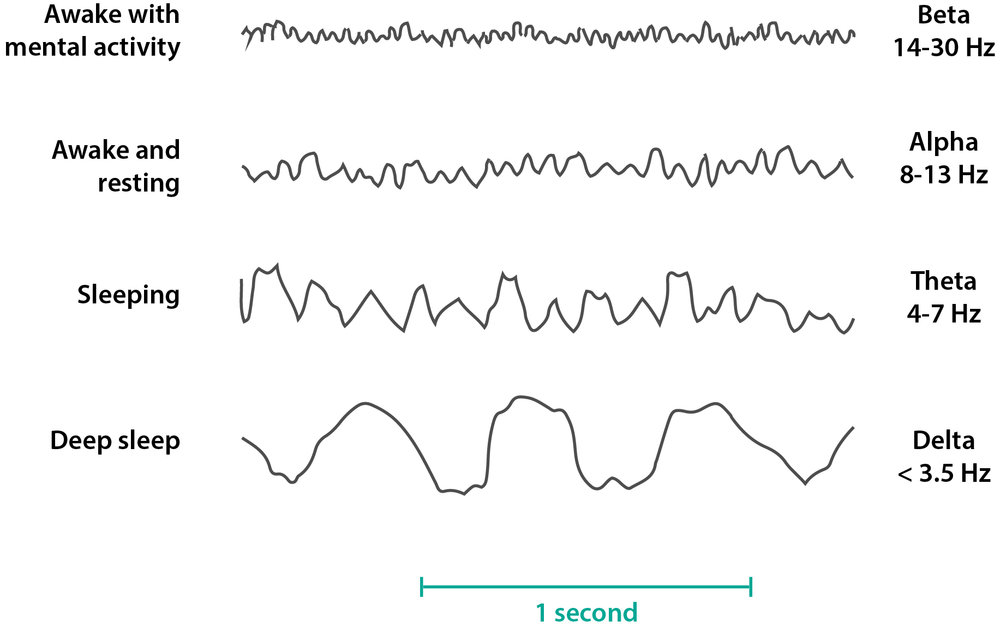
\includegraphics[width=.7\textwidth]{eeg-waves-normal}
    \caption{
امواج مغزی یا سـيگنال‌هاي
\lr{EEG}
 شامل باندهاي متفاوت فركانسي هستند كه هـر يك مرتبط با حالات فيزيكي و شناختي مختلف مي‌باشند.
         }
    \label{fig:eegNormal}
\end{figure}

 الكتروآنسفالوگرافي به حـالات مختلف مغـز (حالات استرس، هوشياري، استراحت و خـواب) حسـاس مي‌باشد. در حالت بيداري عادی با چشم بـاز امـواج بتـا غالب مي‌باشند؛ و در حالت استراحت يا خواب آلودگي امواج آلفا افزايش مـي‌يابـد و در زمان خواب توان فعالیت نوسانی در باندهای فرکانس کمتر افزایش می‌یابد.
% و اگـر خـواب ظـاهر شـود باندهاي با فركانس كم افزايش مي‌يابد. 
 الگوی اموج مغزی منحصربه‌فرد هستند و در برخي موارد ممكن است بتوان بـر اساس فعاليت‌هاي مغزي خاص، آن‌ها را تشخيص داد.
% \cite???
%ریچارد کاتون فعالیت الکتریکی را در نیمکره مغزی خرگوش و میمون کشف کرد و یافته‌هایش را در سال ۱۸۷۵ منتشر کرد. آدولف بک در سال ۱۸۹۰، مشاهدات خود را از فعالیت الکتریکی خودبخودی مغز خرگوش و سگ منتشر کرد که شامل نوسان‌های ریتمیکی می‌شد که توسط نور تغییر یافته و به وسیله الکترودهای سطح مغز تشخیص داده شده بود. قبل از هانس برگر، ولادیمیر ولدیمویوویچ اولین  ثبت نوار مغزی
% حیوانات 
% و توانایی تحریک شده از یک سگ 
% را منتشر کرد.

\section{ ریتم های بهم ریخته در بیماری ها}

\subsection{پارکینسون}
بیماری پارکینسون  ، که با لرزش ، سفتی و کندی حرکت مشخص می شود ، یکی از شایع ترین اختلالات تخریب عصبی در جهان است. مشخصه پاتولوژیک بیماری پارکینسون از دست دادن سلولهای دوپامینرژیک در جسم سیاه
\LTRfootnote{Substantia nigra}
و سایر مناطق مغز است.
مکانیسم‌هایی که باعث از بین رفتن سلول‌های دوپامینرژیک و منجر به بروز نشانه‌های حرکتی بیماری پارکینسون می‌شود هنوز به طور کامل مشخص نشده است. مجموعه‌ای از شواهد در حال رشد، نوسانات عصبی غیر طبیعی درون و بین نواحی مختلف مغز در بیماران پارکینسونی نشان می دهد. 
%پژوهش های متعددی نشان داده اند که بیماری پارکینسون با افزایش فعالیت نوسانی مغز در باند بتا همراه است.

%الگوهای نوسانی منحصر به فردی با ناهنجاری‌های حرکتی خاص در بیماری پارکینسون همراه هستند.
 روش‌های درمانی مانند استفاده از داروهای دوپامینرژیک و تحریک عمقی مغز که این الگوهای نوسانی عصبی غیرطبیعی را مختل می‌کند، باعث بهبود علائم در بیماران علامت می‌شود.

مطالعه فعالیت نورونی هم در انسان و هم در مدل های جانوری بیماری پارکینسون شواهدی در مورد افزایش فعالیت نوسانی در باند بتا در هسته های 
\lr{GPe}
، 
\lr{Gpi} 
و 
\lr{STN}
ارائه کرده است. جالب است که ضایعات یا تحریک هسته های 
\lr{Gpi} 
 و یا
 \lr{STN}
در درمان علائم بیماری پارکینسون موثر هستند، احتمالا به این دلیل که باعث کاهش یا از بین رفتن همگامی غیر طبیعی در خروجی بیزل گنگلیا می شود
\cite{chen2011stimulation, moro2002impact, jenkinson2011new, hammond2007pathological}
.
\subsection{صرع}
صرع رایج ترین اختلال مغزی جدی با شیوع تقریبا کمتر از ۱ درصد کل جمعیت عمومی است.
صرع دربرگیرنده حمله‌های برگشت‌پذیر است که در آن ها فعالیت مغزی با تشدید شدن یا همزمانی گسترده فعالیت های نورون های قشری
\LTRfootnote{cortical neurons}
مختل می شود. 
حمله ها همیشه در نتیجه همزمانی و تشدید نابهنجار و فعالیت ناگهانی یک یا چند توده از نورون‌های‌ قشری رخ می‌دهد. این فعالیت نابهنجار معمولا به روش ثبت موج نمای الکتریکی مغز
\LTRfootnote{EEG}
قابل مشاهده و ثبت است. همزمانی فعالیت سلول‌های عصبی پتانسیل ریتمیک و نسبتا بزرگی ایجاد می‌کند. گرچه بسیاری از افراد مبتلا به صرع، حمله‌های خود را با داروهای در دسترس به شکل موثری مهار می‌کنند، اما گروه کوچکی از این بیماران ممکن است به روش درمانی دیگر، مانند جراحی یا تحریک مغز نیاز داشته باشند.

تحریک عصبی واگ
\LTRfootnote{Vagus Nerve Stimulation (VNS)}
یک تکنیک برای درمان صرع است و یکی از اقدامات نیمه تهاجمی در کنترل تشنج‌ها می‌باشد که در طولانی مدت موجب بهبود کنترل تشنج‌ها می‌گردد. با این روش درمانی تشنج‌ها کمتر و کوتاه‌تر می‌شود و نیاز به درمان دارویی کاهش می‌یابد و در برخی موارد تشنج بیماران بطور کامل از بین می‌رود.

%\subsection{اختلال دوقطبی}
%\subsection{اختلال اوتیسم}

\section{درمان}
برای همه این بیماری‌ها، با توجه به سطح بیماری و پاسخ بیمار به درمان های مختلف، سطوح مختلف درمانی وجود دارد؛ اما در حالت کلی همه درمان‌ها را می توان به سه گونه مختلف تقسیم کرد: درمان‌های رفتاری، درمان‌های شیمیایی، و درمان‌های فیزیکی.

%\begin{itemize}
%  \item درمان‌های رفتاری
%  \item درمان‌های شیمیایی
%  \item درمان‌های فیزیکی
%\end{itemize}

درمان های رفتاری تلاشی برای آموزشِ تنظیم کارکرد درست مغز توسط خود مغز می‌باشد، برای مثال روشی مثل نوروفیدبک
\footnote{بازخورد عصبی یا نوروفیدبک در اصل، نوعی بیوفیدبک است که با استفاده از ثبت امواج الکتریکی مغز و دادن بازخورد به فرد تلاش می‌کند که نوعی خودتنظیمی را به فرد آموزش دهد}
.
درمان های شیمیایی در همه موارد همراه با مصرف دارو یا مواد شیمیایی است که روی کل دستگاه عصبی و یا بخشی از آن اثر می‌گذارد. در درمان‌های فیزیکی اساسا اثرگذاری روی دستگاه عصبی از طریق مکانیزم‌های فیزیکی مختلف اتفاق می‌افتد. تحریک مغز که در این دسته از درمان‌ها قرار دارد به صورت مستقیم روی نرخ فعالیت نورون‌ها تاثیر می گذارد. تمرکز ما بیشتر روی دسته سوم درمان ها  به طور خاص روش های مختلف تحریک مغز و اثرات آن روی شبکه های نورونی خواهد بود.


تحریک مغز به روش های مختلفی انجام می‌گیرد که دسته بندی‌های متفاوتی نیز دارد. برای مثال، از نظر جنس محرک استفاده شده می توان تحریک الکتریکی، تحریک مغناطیسی، تحریک اپتیکی، و تحریک مکانیکی-صوتی را نام برد.
%
%\begin{itemize}
%  \item تحریک الکتریکی
%  \item تحریک مغناطیسی
%  \item تحریک اپتیکی
%  \item تحریک مکانیکی-صوتی
%\end{itemize}

%\subsection{درمان های رفتاری}
%\subsection{درمان های شیمیایی}
%\subsection{اختلال درمان های فیزیکی}

\section{تحریک مغز}

تحریک مغز می تواند به روش های مختلف انجام شود که در دو دسته کلی تهاجمی و غیرتهاجمی جای می‌گیرند. تحریک مغناطیسی فراجمجمه‌ای 
\LTRfootnote{Transcranial Magnetic Stimulation (TMS)}
و تحریک الکتریکی جریان مستقیم فراجمجمه‌ای
\LTRfootnote{Transcranial Direct Current Stimulation (tDCS)}
که کاربرد بیشتری نسبت به سایر روش‌ها دارند، از جمله روش‌های غیرتهاجمی تحریک مغز به شمار می‌روند.
برخی از اشکال مختلف تحریک غیرتهاجمی مغز را می‌توانید در شکل 
\ref{fig:nibs}
ببینید.

\begin{figure}
     \centering
     \begin{subfigure}[t]{0.7\textwidth}
         \centering
         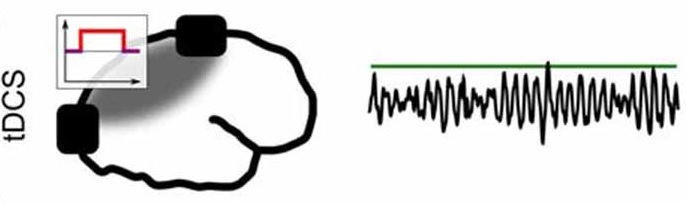
\includegraphics[width=\textwidth]{tdcs}
         \caption{تحریک الکتریکی فرا جمجمه‌ای با جریان مستقیم }
         \label{fig:tdcs}
     \end{subfigure}
     \\
     %\hfill
     \begin{subfigure}[t]{0.7\textwidth}
         \centering
         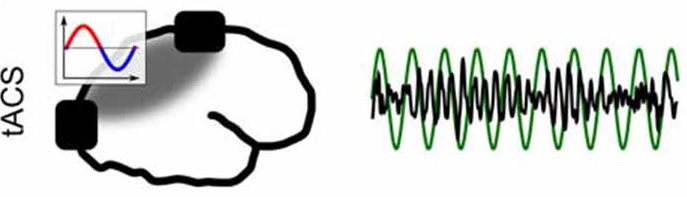
\includegraphics[width=\textwidth]{tacs}
         \caption{    تحریک الکتریکی فرا جمجمه‌ای با جریان متناوب }
         \label{fig:tacs}
     \end{subfigure}
     \\
  %   \hfill
     \begin{subfigure}[t]{0.7\textwidth}
         \centering
         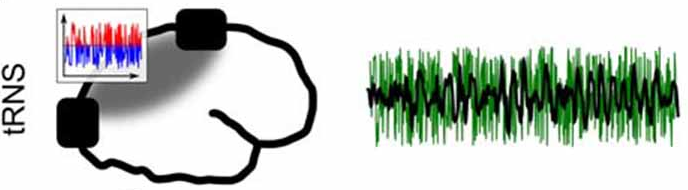
\includegraphics[width=\textwidth]{trns}
         \caption{    تحریک الکتریکی فرا جمجمه‌ای با جریان نویز تصادفی}
         \label{fig:trns}
     \end{subfigure}
     \\
         \begin{subfigure}[t]{0.7\textwidth}
         \centering
         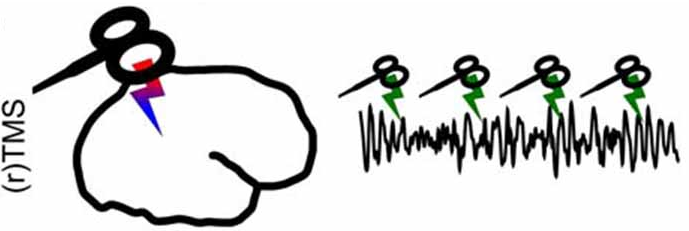
\includegraphics[width=\textwidth]{tms}
         \caption{تحریک مغناطیسی مغز}
         \label{fig:tms}
     \end{subfigure}
        \caption{اشکال مختلف تحریک غیرتهاجمی مغز. تصویر سمت چپ طرحی از نحوه اعمال تحریک و ولتاژ بین الکترودها را با گذشت زمان نشان می دهند. مناطق خاکستری توزیع میدان الکتریکی  در منطقه هدف را نشان می‌دهد. تصویر سمت راست نشان دهنده سیگنال تحریک (سبز) نسبت به  \lr{ EEG }(سیاه) از یک منطقه هدف بالقوه است.
         }
        \label{fig:nibs}
\end{figure}

تحریک مغزی فراجمجمه‌ای و تحریک مغزی عمیق برای درمان طیف وسیعی از بیماری‌های سیستم عصبی و ناهنجاری‌های شناختی از پارکینسون و صرع تا افسردگی، اضطراب و اعتیاد استفاده شده و کارآیی آن مشاهده شده است. با وجود این سازوکار تاثیر تحریک مغزی و علت کارایی آن تقریبا ناشناخته است و عمدتا پروتکل‌های موجود با روش سعی و خطا بوجود آمده و توسعه یافته‌اند. شناخت سازوکار این تاثیرات بر روی دینامیک شبکه‌های عصبی و به طور خاص بر نوسانات جمعی سلول‌های عصبی، برای توسعه هدفمند استفاده از آن‌ها بسیار اساسی است. 


زمینه تحریک غیر تهاجمی مغز در 30 سال گذشته و به ویژه در 15 سال گذشته به طور قابل توجهی توسعه یافته است. مقاله اصلی از بارکر و همکاران 
\cite{barker1985non}
نشان داد كه می‌توان جریان تحریكی را به روش نسبتاً بدون درد با استفاده از تحریک مغناطیسی فرا جمجمه‌ای
 (\lr{TMS}) 
به سیستم عصبی مركزی اعمال کرد. این اتفاق انگیزه فراوانی برای توسعه در این زمینه ایجاد کرده بود. پس از این گزارش مهم، دانشمندان و پزشکان دوباره شروع به بررسی تأثیر بالینی تحریک غیرتهاجمی مغز در ابتدا به عنوان یک روش تشخیصی و سپس به عنوان یک ابزار بالینی کردند.
جالب اینجاست که استفاده از
 \lr{TMS}
به عنوان یک روش تشخیصی آن‌طور که پیش‌بینی می‌شد توسعه نیافت. در پژوهش‌های مختلف نشان داده شده است که
 \lr{TMS}
نقش محدودی به عنوان نشانگر تشخیص بیماری‌های مرتبط با دستگاه عصبی مانند بیماری پارکینسون دارد. با این حال، 
\lr{TMS}
 یا شکل تکراری آن، 
\lr{rTMS}
، با اثرات بالینی قابل توجهی در شرایط اعصاب و روان همراه است
\cite{rossi2009safety}
. در سال 2009 ، این روش توسط سازمان غذا و داروی آمریکا 
\LTRfootnote{US Food and Drug Administration (FDA)}
 به عنوان درمانی برای افسردگی مقاوم 
\LTRfootnote{Refractory depression}
تأیید شد.
پس از علاقه شدید اولیه به 
\lr{TMS}
، دانشمندان این حوزه شروع به بررسی این موضوع کردند که آیا جریان‌های زیاد (مانند جریانهای القا شده توسط 
\lr{TMS}
) برای القای تغییر در شکل‌پذیری عصبی مورد نیاز هستند. این سوال باعث شد دو گروه، یكی در گوتینگن (آلمان) و دیگری در میلان (ایتالیا) به جستجوی یك روش قدیمی تحریک غیرتهاجمی مغز، تحریک جریان مستقیم فراجمجمه‌ای 
\lr{(tDCS)}
بپردازند
\cite{nitsche2008transcranial}.
مطالعات اولیه از این گروه‌ها نشان داد که با توجه به ثابت بودن جهت جریان‌، جریان‌های الکتریکی ضعیف نیز می‌توانند تغییرات قابل توجهی در تحریک‌پذیری قشر ایجاد کنند. این نتایج راه جدیدی را برای کشف مدولاسیون عصبی با جریان های الکتریکی ضعیف باز کرد. در استفاده‌های درمانی برای تقویت اثرات تحریک مغز از ترکیبی از تکنیک‌های مختلف تحریک غیر تهاجمی مغز استفاده می‌شود. با همه این اوصاف، صرف نظر از تعداد قابل توجه مطالعات انجام شده در مورد تحریک غیر تهاجمی مغز، هنوز این پرسش وجود دارد که آیا تاثیر بالینی این روش‌ها معنی دار است؟
%\footnote{معنی دار است یعنی چی؟ از نظر آماری یا از نظر علت و معلولی؟}


تحریک الکتریکی روی یک فیبر عصبی می تواند باعث تولید پتانسیل عمل شود. در این حالت، ولتاژ و یا جریان تحریک باید از آستانه ولتاژ تحریک غشای سلول، بزرگ تر باشد (تحریک بالای آستانه‌ای). یک رویکرد دیگر آن است که ولتاژ غشا سلول عصبی به گونه ای تغییر داده شود که بدون بوجود آمدن پتانسیل عمل، آستانه تحریک‌شوندگی تغییر کند (تحریک زیر آستانه‌ای) که به این وسیله امکان افزایش یا کاهش تحریک‌پذیری سلول فراهم می‌شود.

تحریک الکتریکی جریان مستقیم فراجمجمه‌ای، یک تحریک غیرتهاجمی و زیر آستانه‌ای با هدف ایجاد شرایط مناسب برای تغییر تحریک پذیری عصبی است که در آن معمولاً از دو الکترود صفحه‌ای بزرگ (95-65 سانتی متر مربع) و جریان تقریبا 9 میلی آمپر استفاده می شود. از این روش به عنوان یک راه حل درمانی برای درمان مشکلات عصب شناختی (مانند پارکینسون، سکته مغزی و آلزایمر) و مشکلات روان پزشکی (مانند افسردگی، اختلالات خواب و زوال عقل) استفاده می شود. علاوه بر این، تحقیقات نشان داده است که این روش می تواند موجب ارتقای عملکردهای شناختی مغز مانند توجه، تصمیم گیری، یادگیری، حافظه و شکل‌پذیری سیناپسی در انسان و حیوان شود.

شناخت ساز و کار اثرگذاری انواع مختلف تحریک‌های مغز از این لحاظ حائز اهمیت است که به طراحی پروتکل و سیستم مناسب جهت دست‌یابی به اثر مطلوب از تحریک مغز کمک می‌کند. رویکرد مدل‌سازی که در بسیاری از تحقیقات از آن استفاده شده است می‌تواند در شناخت این ساز و کار موثر باشد. مدل‌سازی فیزیولوژیکی با تجمیع شواهد نوروفیزیولوژیک مختلف قادر به شبیه‌سازی عملکرد نورون‌ها تحت شرایط مورد نظر بوده و به این طریق، شکاف بین کارکرد مشاهده شده از فعالیت عصبی و شواهد آزمایشگاهی که به دلایل فنی (برای مثال دشوار بودن ثبت در سطوح و مقیاس های زمانی مختلف) محدود شده‌اند را برطرف می‌کند. 


\subsection{تحریک عمیق مغز}

%از کتاب پیتر تاس:
%\\
مغز از انبوهی از خوشه‌های نورونی تشکیل شده است که به طرز پیچیده‌ای به هم متصل شده‌اند. این خوشه‌ها با استفاده از اتصالات ساختاری یک یا دو طرفه، گروه‌ها یا حلقه‌هایی را تشکیل می‌دهند. 
در برخی از اختلالات عصبی به عنوان مثال در بیماری پارکینسون، برخی از این خوشه‌های نورونی فعالیت نوسانی غیرعادی و ناهنجار دارند. یکی از راه‌های درمان این بیماری‌ها تحریک عمیق مغز
\LTRfootnote{Deep brain Stimulation (DBS)}
 است.  به مدت بیش از 30 سال تحریک عمیق مغز برای هدف قرار دادن علائم تعدادی از اختلالات عصبی و به ویژه اختلالات حرکتی مانند بیماری پارکینسون و لرزش اساسی  استفاده شده است. در این رهیافت، الکترودهایی با دقت میلی‌متر درون مغز، درون یک خوشه عصبی خاص کاشته می‌شوند. این الکترودها برای سرکوب و تضعیف فعالیت نورونی پاتولوژیک بوسیله تحریک با فرکانس بالا استفاده می‌شوند. چنین درمانی امروزه برای بیمارانی که از بیماری پارکینسون پیشرفته رنج می‌برند و دیگر از درمان‌های دارویی نفعی نمی‌برند استفاده می‌شود. 

در حالی که تحریک عمیق مغز منجر به بهبود علائم در بسیاری از بیماران می شود، مکانیسم های اساسی این بهبود به روشنی درک نشده است و تاکنون مشخص نیست که چگونه این نوع تحریک، فعالیت نورونی ریتمیک که باعث ایجاد لرزش در بیماران پارکینسونی می‌شود را سرکوب می‌کند؛ به همین دلیل معتقدیم که درک صحیح نظری از رفتار دینامیکی خوشه های نورونی در پاسخ به تحریک می‌تواند به بهبود تکنیک‌های تحریک کمک کند.

تحریک عمقی مغز نوعی روش درمانی (جراحی) در پزشکی است که در طی آن الکترودهایی در داخل مغز بیمار قرار داده می‌شوند. این الکترودها پس از کاشته شدن در مغز به یک دستگاه مولد پالس الکتریکی
 \LTRfootnote{Pulse Generator}
  متصل می‌شوند. پالس الکتریکی تولید شده توسط دستگاه مولد پالس از طریق الکترودهای کاشته شده در مغز به بافت‌های عمقی مغز انتقال یافته و از این طریق اثر درمانی خود را اعمال می‌نماید. روش درمانی تحریک عمقی مغز برای اولین بار در انسان در سال ۱۹۸۷ توسط جراح مغز و اعصاب فرانسوی علیم-لویی بن عبید
\LTRfootnote{Alim-Louis Benabid}
به کار گرفته شد. سیستم تحریک عمقی مغز سه بخش دارد که درون بدن نصب می شوند:
\begin{itemize}
\item تحریک‌کننده عصبی یا مولد پالس: دستگاهی ضربان ساز و قابل برنامه ریزی است که با باتری کار می‌کند و باعث تولید پالس های الکتریکی می‌شود. این دستگاه زیر پوست قفسه سینه یا شکم قرار می‌گیرد (شکل 
\ref{fig:dbs00}
).
\item سیم های انتقال جریان: سیم هادی که لیدها را به تحریک‌کننده متصل می‌کنند. این سیم معمولاً در زیر پوست جایگذاری می‌شود و از جمجمه به پشت گوش و گردن و نهایتا به سینه می‌رسد (شکل 
\ref{fig:dbs00}
).
\item لید: یک سیم با تعدادی الکترود در نوک آن است که پالس های الکتریکی را به بافت مغزی منتقل می کند. الکترودها درون مغز قرار می‌گیرند و از یک سوراخ کوچک در جمجمه به سیم‌ها متصل شده‌اند (شکل 
\ref{fig:dbs01}
).
\end{itemize}

\begin{figure}[h!]
    \centering
     \begin{subfigure}[t]{0.45\textwidth}
         \centering
         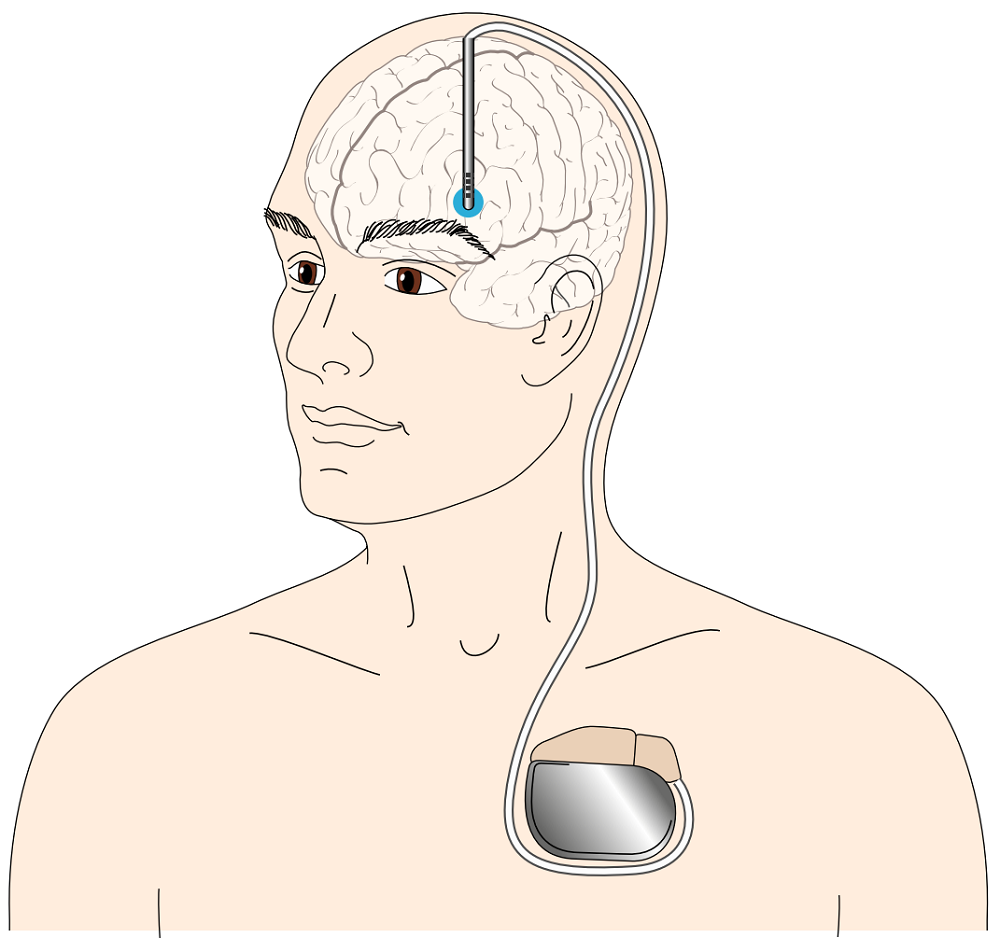
\includegraphics[width=\textwidth]{dbs00}
         \caption{
         الکترودها و تولید کننده های پالس به طور دائمی کاشته می شوند. 
         بسته به نوع علائم ، می توان الکترودها را در یک یا هر دو نیمکره مغز کاشت.
         الکترود (های) کاشته شده در مغز به دستگاه ضربان‌ساز کاشته شده در قفسه سینه متصل است.
         }
         \label{fig:dbs00}
     \end{subfigure}
    \
         \begin{subfigure}[t]{0.45\textwidth}
         \centering
         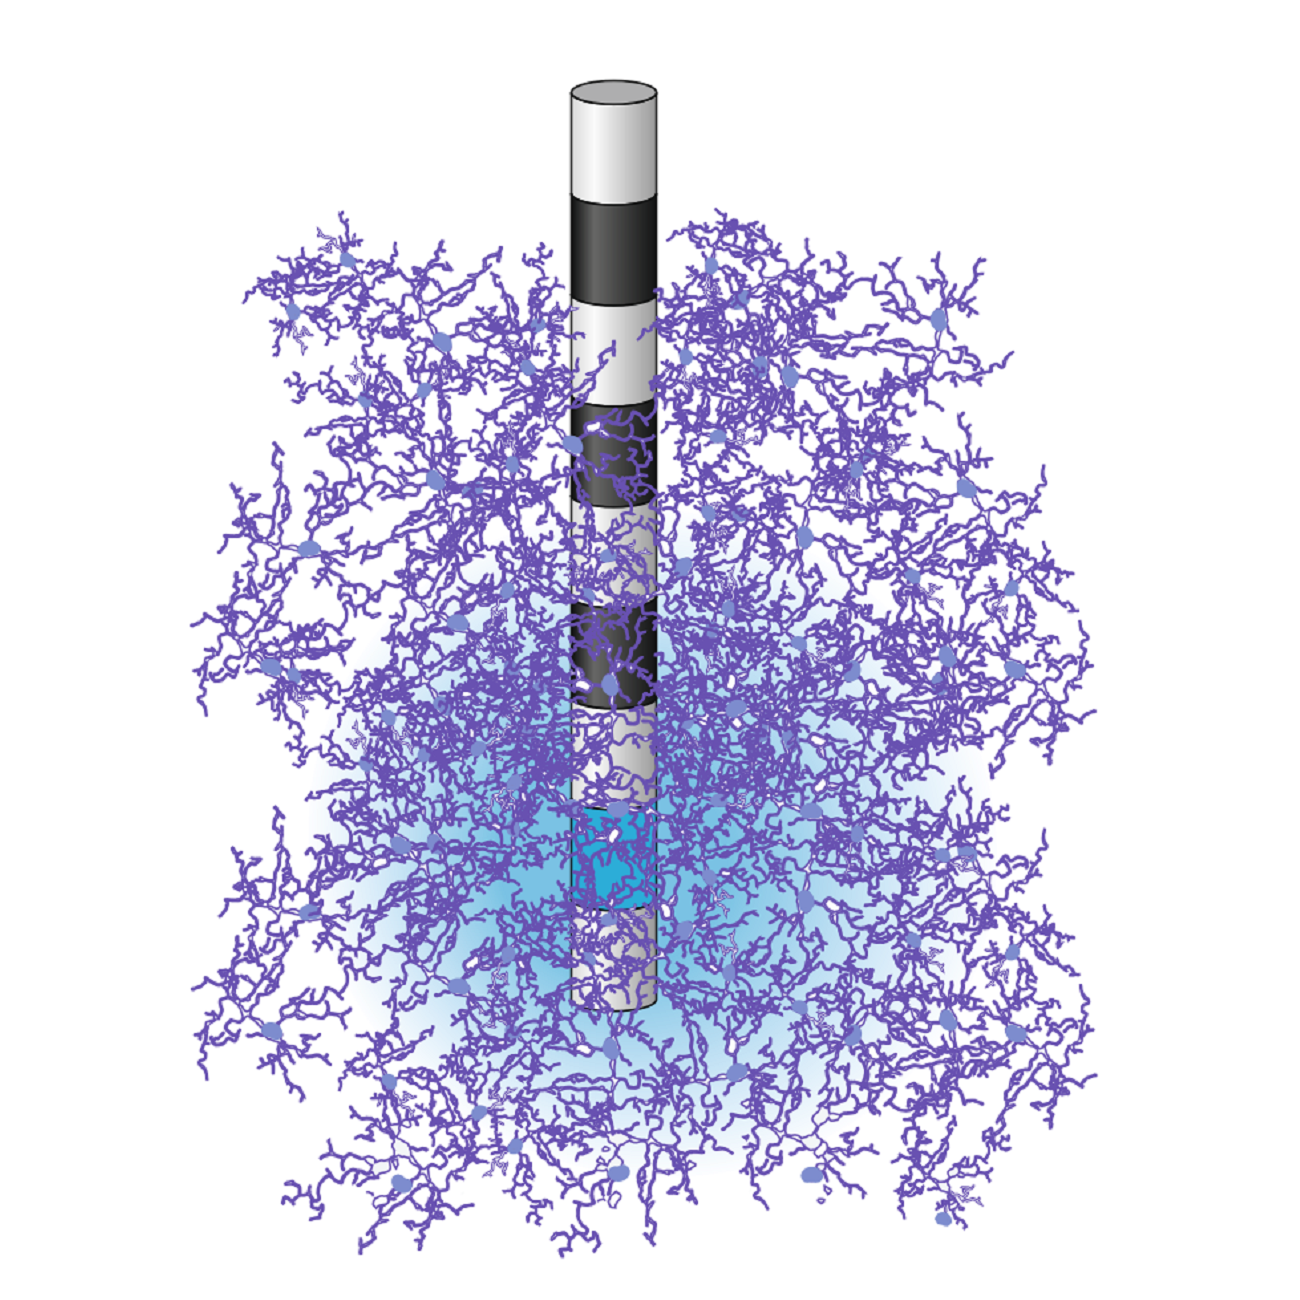
\includegraphics[width=\textwidth]{dbs01}
         \caption{  
         الکترودهای تحریک عمیق مغز سنتی از چهار نقطه تماس (استوانه‌های سیاه) تشکیل شده است، که معمولاً از یکی از این نقاط تماس برای تحریک استفاده می‌شود. متداول‌ترین هدف جراحی برای درمان بیماری پارکینسون‌، هسته زیر تالاموس است که تقریبا حاوی 250000 نورون که با رنگ آبی به تصویر کشیده شده و در واقع بسیار متراکم‌تر از چیزی است در تصویر می‌بینید.
         }
         \label{fig:dbs01}
     \end{subfigure}
     \caption{طرحی از تحریک عمیق مغزی }
    \label{fig:dbs}
\end{figure}


در شکل 
\ref{fig:dbs}
طرحی از تحریک عمیق مغزی و اجزا مختلف آن می‌بینید و در شکل
\ref{fig:dbs-xray}
تصویر رادیولوژی از الکترودها و نوسان‌سازی به کمک جراحی در مغز و بدن بیمار قرار داده شده‌اند.

\begin{figure}[h!]
     \centering
     \begin{subfigure}[t]{0.3\textwidth}
         \centering
         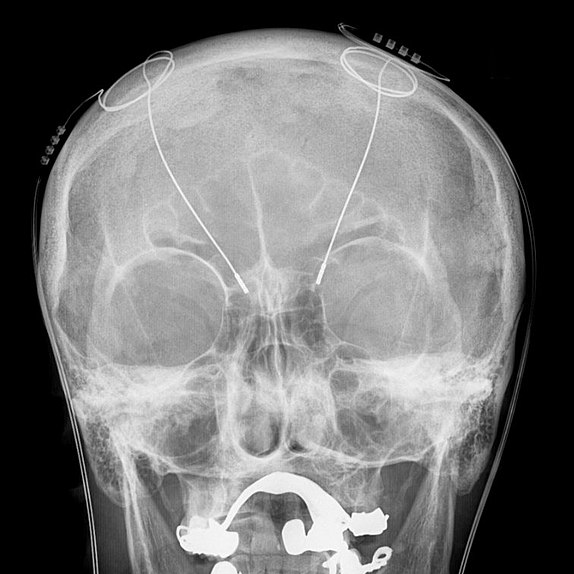
\includegraphics[width=\textwidth]{dbs-xray-1}
         \caption{الکترودهای تحریک عمیق مغز کاشته شده در سر }
%         \label{fig:tdcs}
     \end{subfigure}
     \
     %\hfill
     \begin{subfigure}[t]{0.3\textwidth}
         \centering
         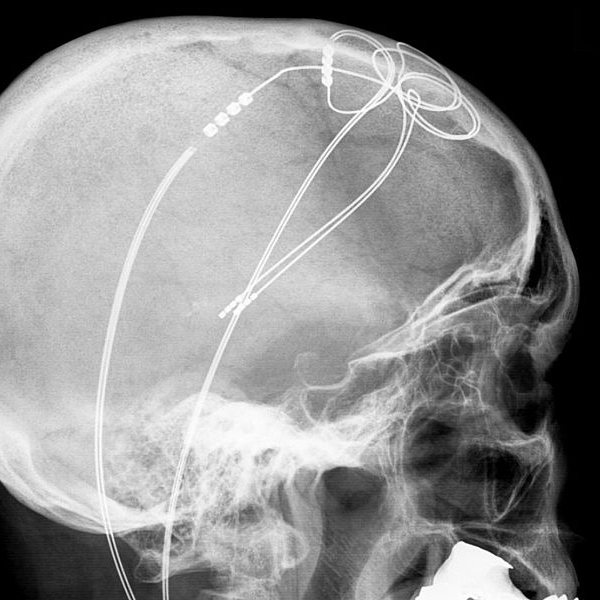
\includegraphics[width=\textwidth]{dbs-xray-2}
         \caption{الکترودهای تحریک عمیق مغز کاشته شده در سر }
%         \label{fig:tacs}
     \end{subfigure}
     \
  %   \hfill
     \begin{subfigure}[t]{0.3\textwidth}
         \centering
         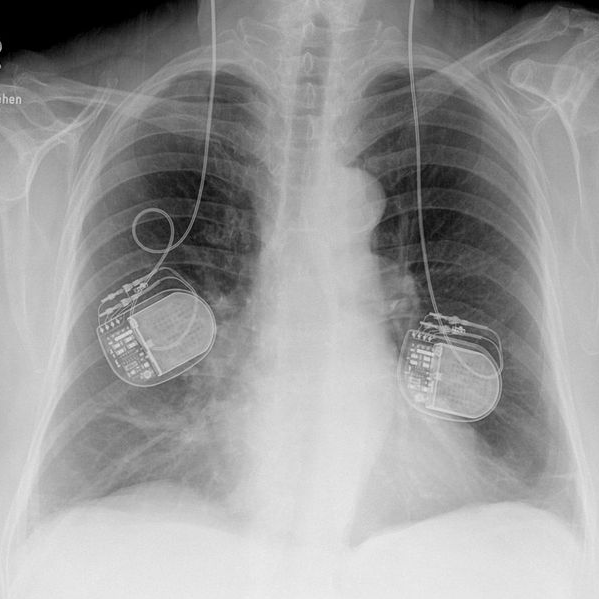
\includegraphics[width=\textwidth]{dbs-xray-3}
         \caption{    نوسان‌سازهای کار گذاشته شده درون قفسه سینه}
%         \label{fig:trns}
     \end{subfigure}
        \caption{
تصویر رادیولوژی سر و قفسه سینه فردی بعد از کاشت الکترودهای تحریک عمیق مغز.
         }
        \label{fig:dbs-xray}
\end{figure}
%
%از مقاله ها:
%\\


%می‌دانیم که از دست دادن نورون‌های دوپامینرژیک در توده سیاه
%\LTRfootnote{Substantia nigra}
% منجر به بیماری پارکینسون می‌شود، در حالی که تأثیر دقیق این امر بر دینامیک مغز کاملاً مشخص نیست، با این حال در بیماران مبتلا به پارکینسون فعالیت نوسانی غیر عادی در باند بتا مشاهده شده است.

%با اینکه علت  لرزش اساسی هنوز ناشناخته است، با این حال، نوسانات پاتولوژیک در شبکه تالاموکورتیکال-مخچه با لرزش مرتبط است.

%هر دو این اختلالات حرکتی با تحریک عمیق مغز درمان می شوند ، که لازمه این امر کاشت الکترود در مغز بیمار می‌باشد. 

\section{   مدلسازی نوسانات عصبی در شبکه‌های نورونی }

%\subsection{نوسانگرها}
نوسانگرها در فیزیک و در دیگر علوم طبیعی  مانند شیمی و زیست شناسی بسیار فراوان‌اند.
امروزه بررسی نوسانگر‌ها شاخه مهمی از فیزیک غیرخطی می‌باشد که باعث درک بهتر ما از برهمکنش نوسانگر‌ها و واکنش یک نوسانگر به اختلالات خارجی شده است.
برای مثال، اثر تحریک ضربان‌دار
\LTRfootnote{Pulsatile stimulus}
روی یک نوسانگر منفرد با جزییات بررسی شده است. 
از آنجا که می‌توان نورون‌ها را به عنوان یک نوسانگر مدلسازی کرد؛ این دانش برای مطالعه واکنش یک نورون منفرد به تحریک‌های الکتریکی ضربان‌دار دارای اهمیت بسیاری است.
بِست
\LTRfootnote{Best}
به صورت نظری پاسخ فاز
\LTRfootnote{phase resetting}
یک نورون منفرد را تحلیل کرد.
\cite{best1979disrupting}
او اثر تحریک را روی دینامیک فاز نورون که توسط رابطه بین فاز قبل و بعد از اعمال یک تحریک ضربان‌دار مشخص می‌شود را بررسی کرد. در میان تعدادی اثر دیگر، او پیش بینی کرد که توسط یک محرک الکتریکی به موقع، با شدت و مدت زمان مناسب می‌توان شلیک تکراری یک آکسون را متوقف کرد. این پیش‌بینی‌ها به صورت آزمایشگاهی توسط گاتمن، لوییز و رینزل تایید شدند.
\cite{guttman1980control}
بعلاوه، تعداد زیادی آزمایش روی حیوانات انجام شد که به وضوح نشان می‌دهد که همگامی فعالیت عصبی نوسانی مکانیزمی اساسی برای ترکیب اطلاعات مرتبط درون نواحی مغز و همچنین بین نواحی مختلف است؛ و پیش از این نیز اشاره گردید که همگامی نورون‌ها نقش مهمی در شرایط پاتولوژیک بازی می‌کند؛ برای مثال در دوره‌های لرزش یا حمله‌های صرعی. به همین علت و برای مطالعه این موارد رفتار جمعیت‌های نورونی در کانون توجه قرار گرفت. 

این که بفهمیم چگونه یک تحریک روی فعالیت همگام نورون‌ها تأثیر می‌گذارد از اهمیت بالایی برخوردار است. از یک جهت تحریک ابزار آزمایشگاهی مهمی برای بررسی و مطالعه فرآیندهای همگام نورونی است. برای مثال، تحریک حسی طبیعی برای بررسی پردازش اطلاعات نورونی استفاده می‌شود. در حالی که تحریک الکتریکی و مغناطیسی سیستم عصبی در آزمایشگاه برای تحلیل بر همکنش دینامیکی نواحی مختلف مغز بکار می‌رود. از سوی دیگر، امروزه تحریک عمیق مغز یک روش درمانی امیدوار کننده است، مثلا برای بیمارانی که از پارکینسون پیشرفته رنج می‌برند و به درمان‌های دارویی پاسخ نمی‌دهند. 

دانش مربوط به تحریک فعالیت‌های همگام نورونی به طور عمده بر پایه نتایج آزمایشگاهی و مشاهدات کلینیکی است. بر این اساس، می توان انتظار داشت که درک نظری عمیق‌تری از پدیده‌‌های دینامیکی مربوطه ممکن است هم مطالعه عملکرد مغز و هم تکنیک‌های تحریک درمانی را بهبود بخشد. به عنوان مثال، درک پاسخ‌های گذرای مشخصه
\LTRfootnote{characteristic transient responses}
یک جمعیت نورونی به اختلالات خارجی، ممکن است سرنخ‌های بسیار مهمی برای بررسی چگونگی واکنش و انطباق سیستم عصبی مرکزی با شرایط خارجی‌ای که به سرعت در حال تغییر هستند ، در اختیار ما قراردهد. با این حال، برای کاربردهای درمانی، طراحی یک تکنیک تحریک برای ازبین بردن همگامی که  با وجو عوارض جانبی کم تا حد ممکن موثر باشد، یک چالش بزرگ است. تحقیقات نظری در مورد رفتارهای تجمعی خودبخودی در مجموعه‌ای از نوسانگرهای جفت شده نتایج قابل توجهی را آشکار کرده است. با این حال، هنوز هم نیاز زیادی به مطالعات مربوط به تأثیر تحریک بر گروهی از نوسانگرها وجود دارد.

بر این اساس، این پژوهش سه هدف اصلی دارد: 
۱- بررسی فرآیند های همگام سازی و ناهمگام سازی ناشی از تحریک در سیستم های نورونی؛ ۲- رسیدن به یک چارچوب نظری برای تفسیر رفتار دینامیکی ناشی از تحریک جمعیت های نورونی؛ ۳- ارایه مبانی نظری برای بهبود و طرای تکنیک های تحریک برای درمان بیماری های مختلف.

در بدن انسان ریتم‌های فیزیولوژیک متعددی وجود دارد که در مقیاس زمانی گسترده‌ای از یک میلی‌ثانیه تا ماه اتفاق می‌افتد. به عنوان مثال، فعالیت‌های نورونی، ضربان قلب، تنفس، گردش خون، متابولیسم انرژی در سلول‌ها، رفتارهای حرکتی تکراری (راه رفتن، دویدن، پرواز کردن، شنا و جویدن)، چرخه های خواب، رشد فصلی. در این زمینه، اصطلاح ریتم به معنی عمل جمعی هماهنگ جمعیت‌هایی از زیر سیستم‌های نوسانی، برای مثال نورون های نوسانی، است.
انواع مختلفی از فعالیت های ریتمیک در مناطق مختلف مغز مشاهده می‌شود. این ریتم‌ها نقش مهمی در فرآیندهای فیزیولوژیکی و همچنین آسیب شناختی مانند کنترل حرکت و لرزش دارند. 

در دهه گذشته، تعداد زیادی از آزمایشات روی حیوانات به برهمکنش نورون‌ها در یک خوشه و بین خوشه‌های واقع در مناطق مختلف مغز پرداخته است. در هر دو مورد، همگام‌سازی به معنی شلیک همزمان، مکانیزم اساسی برای ترکیب پردازش‌های نورونی‌ای است که ممکن است به طور گسترده‌ای در مغز توزیع شود.

تحریک در مورد فرآیند‌های تنظیمی و همگام‌سازی از اهمیت زیادی برخوردار است:
۱- تحریک حسی طبیعی: مغز بطور دائم در معرض سیل اطلاعات دریافتی قرار دارد. به طور مداوم ورودی‌های حسی بی شماری باید به سرعت ارزیابی شوند تا اینکه رفتار بتواند با تغییرات محیطی سازگار باشد. برای بررسی پردازش اطلاعات حسی مغز، محرک‌های مختلفی مانند صدا و نور اعمال می‌شوند و فعالیت مغزی برانگیخته شده توسط 
\lr{EEG}
یا 
\lr{MEG}
ثبت می‌شود. به این ترتیب نقش مناطق مختلف مغز در پردازش اطلاعات حسی به طور دقیق مورد مطالعه قرار گرفت. 

از طرف دیگر تغییرات مشخصه پاسخ مغز به تحریک‌های حسی راهنماهای تشخیصی ارزشمندی هستند. 
۲- تحریک الکتریکی و مغناطیسی آزمایشگاهی: امروزه نمی‌توان بدون استفاده از تحریک، نوسانگرهای نورونی جفت شده را مطالعه کرد. با توجه به این هدف، فردی تحریکی را به حجم کمی از بافت مغز اعمال می‌کند و تغییرات حاصل از فعالیت مغز و رفتار مربوطه را مشاهده می‌کند. معاینات و آزمایش‌های از این نوع در آزمایشات روی حیوانات و در بیماران هنگام جراحی مغز و اعصاب انجام می‌شود. علاوه براین، در عصب‌شناسی تحریک برای اهداف تشخیصی و همچنین درمانی اعمال می‌شوند. 


%\subsection{مدلسازی تک نورون}
%\subsection{مدل های جمعیتی -\lr{Mass models}}
\subsection{ مدل کوراموتو به عنوان یک مدل جمعیتی ساده  }

مدل کوراموتو از نوسانگرهای فاز یکی از مدل‌های انتزاعی و اساسی مورد استفاده برای بررسی نوسانات عصبی و همگام‌سازی است.
داده های نوسانی که ما با آن درگیر هستیم ناشی از فعالیت الکتریکی همبسته جمعیت های عصبی است.
به منظور توصیف چنین سیستم هایی ، ما از یک مدل نوسانگر جفت شده استفاده می کنیم که تحول زمانی مجموعه ای از 
$N$
نوسانگر توسط معادلات کوراموتو مشخص می شود که دارای یک جمله اضافی برای توصیف اثرات تحریک می باشد.

\begin{equation}
    \frac{d \theta_i}{dt} = \omega_i + \frac{k}{N} \sum_{j=1}^{N} \sin(\theta_j -\theta_i) + I \delta(t-t_{stim}) Z(\theta_i)
    \label{eq:kuramotoModel}
\end{equation}
جمله اول، 
$\omega_i$
فرکانس طبیعی نوسانگر 
$i$ 
ام می‌باشد.
جمله دوم توصیف کننده برهمکنش بین نوسانگرهای مختلف است که 
$k$
ضریب جفت شدگی می‌باشد و قدرت جفت‌شدگی بین هر جفت نوسانگر و در نتیجه تمایل نوسانگرها برای همگامی را کنترل می‌کند. 
جمله سوم اثر تحریک را توصیف می‌کند؛ شدت تحریک توسط 
$I$
مشخص شده است و تابع 
$\delta(t-t_{stim})$
در همه زمان‌ها صفر است به جز در زمان‌هایی که تحریک اعمال می‌شود که برابر است با یک.
تابع پاسخ فاز یک نوسانگر منفرد نیز
$Z(\theta_i)$
است.

پارامتر نظم برای مجموعه ای از نوسانگر ها به صورت زیر تعریف می شود
\begin{equation}
    r=\frac{1}{N} \sum_{j=1}^{N} e^{i \theta_j}
    \label{eq:orderParam}
\end{equation}
کاملا واضح است که 
$r$
یک عدد مختلط است و می توان آن را به صورت 
\begin{equation}
    r=\rho e^{i \psi}
    \label{eq:orderparamComplex}
\end{equation}
نوشت. 
اندازه 
$\rho$
معیاری از همگامی است؛ که مقادیر صفر و یک آن به ترتیب با حالت کاملا ناهمگام و حالت کاملا همگام متناظر هستند. به کمک رابطه اویلر می توان پارامتر نظم را به صورت زیر بازنویسی کرد
\begin{equation}
    \rho e^{i \psi} = \frac{1}{N} \sum_{n=1}^{N} \cos [\theta_n(t)] + i \frac{1}{N} \sum_{n=1}^{N} \sin [\theta_n(t)].
    \label{eq:orderParamExpansion}
\end{equation}
به کمک تعریف پارامتر نظم (معادله
\ref{eq:orderparamComplex}
)
می توان معادله تحول نوسانگرهای کوراموتو (معادله
\ref{eq:kuramotoModel}
)
را به صورت زیر بازنویسی کرد
\begin{equation}
      \frac{d \theta_l}{dt} = \omega _l + k \rho \sin ( \psi - \theta_l) + I \delta(t-t_{stim}) Z(\theta_l).
\end{equation}
با نوشتن معادلات به این شکل، واضح است که هر نوسانگر تمایل دارد به سمت فاز جمعیت،
$\psi$
، حرکت کند و این تمایل توسط ضریب جفت شدگی، 
$k$
،کنترل می شود.


\subsection{تابع پاسخ فاز}
با اعمال اختلال به یک نوسانگر و اندازه‌گیری اثر آن روی طول دوره نوسان می‌توان نمودار پاسخ فاز
\LTRfootnote{Phase Response Curve (PRC)}
 نوسانگر را بدست آورد. با توجه به شکل
 \ref{fig:prc}
پاسخ فاز نوسانگر را به صورت زیر تعریف می کنند:
\begin{equation}
\Delta \phi = (T_0 - T_1)/T_0
\label{eq:prc}
\end{equation}


\begin{figure}[h!]
	\centering
	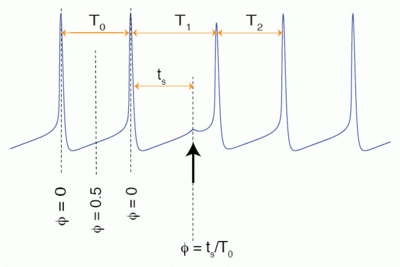
\includegraphics[width=0.5\textwidth]{prc}
    \caption{
با اعمال اختلال به یک نوسانگر و اندازه‌گیری اثر آن روی طول دوره نوسان می‌توان نمودار پاسخ فاز نوسانگر را بدست آورد.
\label{fig:prc}
    }
%    \label{fig:dbs-protocols}
\end{figure}

  نورون‌ها بر اساس تابع پاسخ فاز به دو دسته تقسیم می‌شوند. در نوع اول، با وارد کردن اختلال در هر لحظه‌ای فاز جلو می‌افتد؛ اما در نوع دوم، بر اساس لحظه اعمال اختلال فاز ممکن است جلو یا عقب بیفتد.
  
\begin{figure}
	\centering
	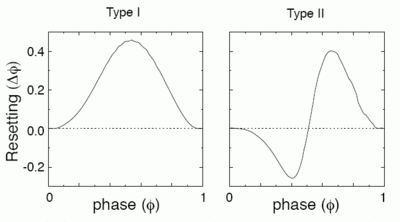
\includegraphics[width=0.5\textwidth]{prc-types}
    \caption{
  نورون‌ها بر اساس تابع پاسخ فاز به دو دسته تقسیم می‌شوند. در نوع اول، با وارد کردن اختلال در هر لحظه‌ای فاز جلو می‌افتد؛ اما در نوع دوم، بر اساس لحظه اعمال اختلال فاز ممکن است جلو یا عقب بیفتد.
    }
%    \label{fig:dbs-protocols}
\end{figure}

  
  
  
  
  
  
  
  
  
  
  
  
  
  
  
  
  
  
  
  
  
  
\section{نتایج }
\subsection{تضعیف وابسته به فاز نوسانات غیر عادی در سیستم عصبی}
همان‌طور که تا کنون اشاره شد بیماری‌های مختلفی هستند که با افزایش غیر طبیعی نوسانات مغزی همراه هستند. 
 یکی از راه‌های درمانی برای مقابله با این شرایط استفاده از تحریک عمیق مغز می‌باشد. تحریک عمیق مغز به وسیله الکترودهایی که درون بافت مغز قرار می‌گیرند، اعمال می‌شود.

\begin{figure}
	\centering
	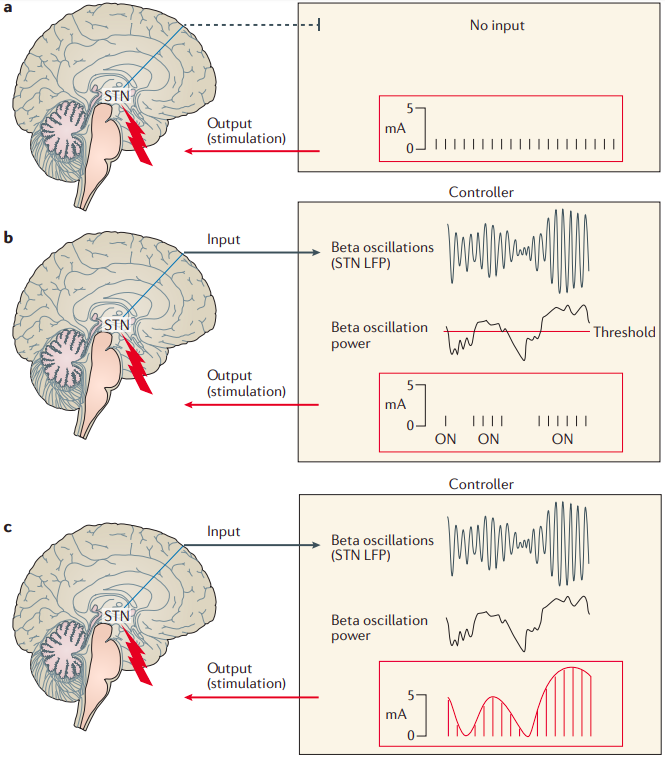
\includegraphics[width=0.9\textwidth]{dbs-protocols}
    \caption{
    پروتکل‌های مختلف در اعمال تحریک عمیق مغز.
در شکل بالایی تحریک عمیق مغز حلقه-باز را می‌بینیم؛ در این پروتکل پارامترهای تحریک ثابت هستند. 
در شکل میانی، بر اساس پایش و نظارت تنها یک پارامتر از سیگنال ورودی (در اینجا توان سیگنال ورودی)، خروجی دستگاه نوسان‌ساز را تعیین می‌کند. در پروتکل نشان داده شده در شکل میانی، تنها در صورتی که توان امواج بتا از آستانه مشخصی بیش‌تر شود، تحریک هایی با دامنه و فرکانس ثابت به مغز اعمال می‌شود. اما در شکل پایین بیش از یک مشخصه از سیگنال ورودی روی تعیین نحوه و مشخصات اعمال تحریک اثر می‌گذارد. مثلا در همین شکل، قدرت تحریک نیز بر اساس قدرت سیگنال ورودی تنظیم می‌شود.
    }
    \label{fig:dbs-protocols}
\end{figure}


پس از کاشت الکترود، برای تضعیف نشانه‌های پاتولوژیک و ایجاد اثرات جانبی کمتر باید پارامترهای تحریک نظیر فرکانس تحریک و شکل موج تحریک تنظیم شوند. به کمک مدل‌های محاسباتی می‌توان پارامترهای بهینه تحریک عمیق مغز را تخمین زد. در طول سال‌های گذشته پروتکل‌های مختلفی برای نحوه اعمال تحریک‌ها ارایه شده است که برخی از آن‌ها در شکل
\ref{fig:dbs-protocols}
نمایش داده شده‌اند. 

پروتکل‌هایی که در آن‌ها پارامترهای تحریک ثابت باشند تحریک عمیق مغز حلقه-باز نامیده می‌شوند.
 از منظر فرکانسی، تحریک عمیق مغز حلقه-باز دو دسته دارد. اگر فرکانس اعمال تحریک از ۱۰۰ هرتز کمتر باشد، فرایند تحریک در دسته تحریک عمیق مغز فرکانس پایین جای می‌گیرد و اگر فرکانس تحریک بیشتر از ۱۰۰ هرتز باشد فرآیند تحریک در دسته تحریک عمیق مغز با فرکانس بالا قرار می‌گیرد. اگر تحریک عمیق مغز با پارامتر‌های غیر ثابت، واکنشی و براساس فعالیت در حال وقوع در مغز اعمال شود، تحریک عمیق مغز حلقه-بسته نامیده می‌شود. تحریک حلقه-بسته را می‌توان بر اساس  پایش و نظارت تعداد متفاوتی از نشانگرهای مختلف اعمال کرد. این رهیافت می‌تواند اثرات جانبی را کاهش داده و اثربخشی درمان را افزایش می‌دهد.
 
\begin{figure}[t!]
     \centering
     \begin{subfigure}[t]{0.45\textwidth}
         \centering
         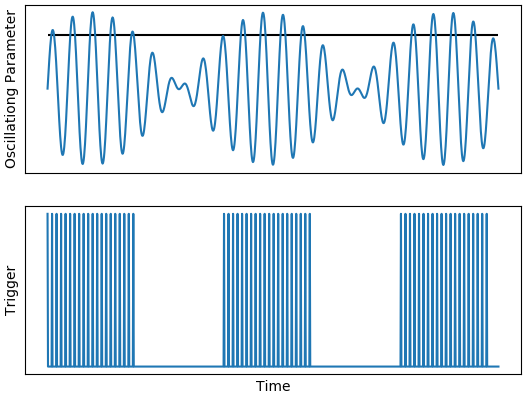
\includegraphics[width=\textwidth]{dbs-closedloop1}
         \caption{
 اعمال تحریک بر اساس دامنه فعالیت نوسانی در حال انجام در مغز.
         }
%         \label{fig:tdcs}
     \end{subfigure}
     \
     %\hfill
     \begin{subfigure}[t]{0.45\textwidth}
         \centering
         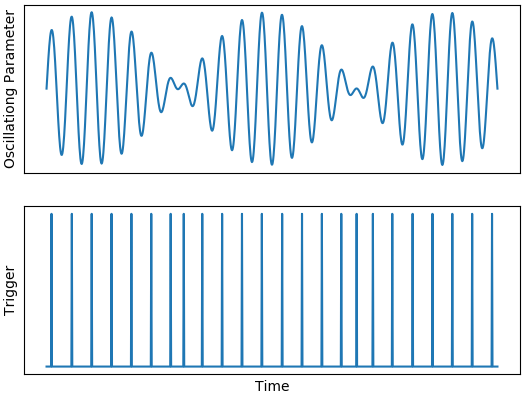
\includegraphics[width=\textwidth]{dbs-closedloop2}
         \caption{
 اعمال تحریک بر اساس فاز فعالیت نوسانی در حال انجام در مغز.
         }
%         \label{fig:tacs}
     \end{subfigure}
        \caption{
دو پروتکل معروف در رهیافت حلقه-بسته
         }
        \label{fig:dbs-closed-loop}
\end{figure}



پارامترهای شکل موج از پارامترهای مهم در تحریک عمیق مغز می‌باشد. برخی از گروه‌های پژوهشی به بررسی نحوه اثر و پیدا کردن پارامترهای بهینه شکل موج می‌پردازند. تعریف دقیق پارامترهای شکل موج در تحریک عمقی مغز می‌تواند از آسیب دیدن بافت مغز یا الکترود جلوگیری کند، فعالیت عصبی را افزایش داده و هزینه انرژی را کاهش دهد که باعث افزایش عمر باتری می‌شود و از این رو از جراحی‌های جایگزینی دستگاه جلوگیری می‌شود. در شکل 
\ref{fig:dbs-pulse-shape}
می‌توانید نمونه‌هایی از شکل موج‌های مختلف را مشاهده کنید. 


\begin{figure}[b!]
     \centering
     \begin{subfigure}[t]{0.3\textwidth}
         \centering
         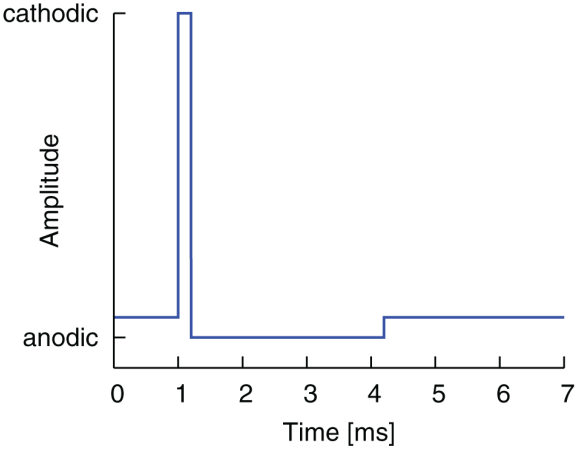
\includegraphics[width=\textwidth]{pulse-shape1}
%         \caption{الکترودهای تحریک عمیق مغز کاشته شده در سر }
%         \label{fig:tdcs}
     \end{subfigure}
     \
     %\hfill
     \begin{subfigure}[t]{0.3\textwidth}
         \centering
         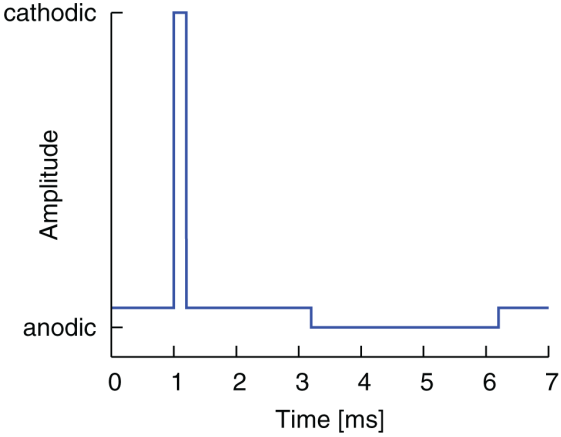
\includegraphics[width=\textwidth]{pulse-shape2}
%         \caption{الکترودهای تحریک عمیق مغز کاشته شده در سر }
%         \label{fig:tacs}
     \end{subfigure}
     \
  %   \hfill
     \begin{subfigure}[t]{0.3\textwidth}
         \centering
         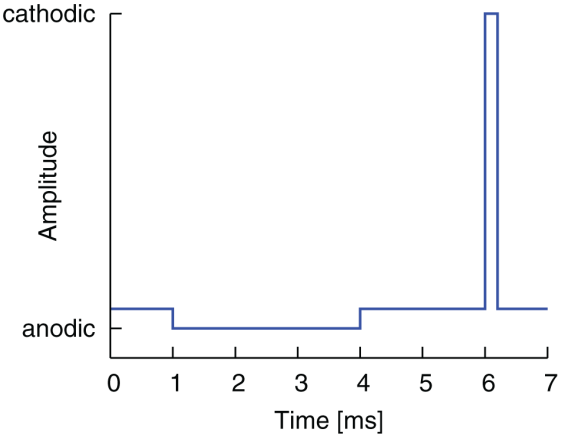
\includegraphics[width=\textwidth]{pulse-shape3}
%         \caption{    نوسان‌سازهای کار گذاشته شده درون قفسه سینه}
%         \label{fig:trns}
     \end{subfigure}
        \caption{
شکل موج‌های مختلف در تحریک عمیق مغز که بین قسمت‌های آنُدیک و کاتُدیک تاخیر متفاوتی دارند.
         }
        \label{fig:dbs-pulse-shape}
\end{figure}



موفقیت تحریک عمیق مغز حلقه-بسته به طراحی استراتژی تحریک بستگی دارد که بر اساس آن نوسانات عصبی تضعیف می‌شوند. یک گام مهم در این راستا، ساختن مدلی ریاضی است که بتواند پاسخ نوسانات عصبی به تحریک در حالت‌های مختلف مغز را توصیف کند.
ما در بررسی‌های اولیه جمعیت نورونی که نوسانات پاتولوژیک تولید می‌کند را با شبکه‌ای از نوسانگرهای جفت شده مدل‌سازی کردیم. معادله تحول این نوسانگرها بر اساس مدل کوراموتو نوشته شده‌است. همچنین تحریک‌ها در یک لحظه خاص وقتی که فاز سیستم مقدار مشخصی است به اندازه تابع پاسخ فاز هر نوسانگر به آن‌ها وارد می‌شود.
رفتار وابسته به زمان مدل کوراموتو به صورت عددی در شبکه کامل مورد مطالعه قرار گرفته است. ما رفتار ناهمگام شدن را با حل این مدل روی شبکه کامل بررسی کردیم.
\begin{equation}
    \frac{d \theta_i}{dt} = \omega_i + \frac{k}{N} \sum_{j=1}^{N} \sin(\theta_j -\theta_i) + I \delta(t-t_{stim}) Z(\theta_i)
    \label{eq:kuramotoModelres}
\end{equation}
جمله اول، 
$\omega_i$
فرکانس طبیعی نوسانگر 
$i$ 
ام می باشد.
جمله دوم توصیف کننده برهمکنش بین نوسانگرهای مختلف است که 
$k$
ضریب جفت شدگی می‌باشد و قدرت جفت شدگی بین هر جفت نوسانگر و در نتیجه تمایل نوسانگرها برای همگامی را کنترل می کند. 
جمله سوم اثر تحریک را توصیف می کند؛ شدت تحریک توسط 
$I$
مشخص شده است و تابع 
$\delta(t-t_{stim})$
در همه زمان ها صفر است به جز در زمان هایی که تحریک اعمال می‌شود که برابر است با یک.
تابع پاسخ فاز یک نوسانگر منفرد نیز
$Z(\theta_i)$
است.

\begin{figure}
	\centering
	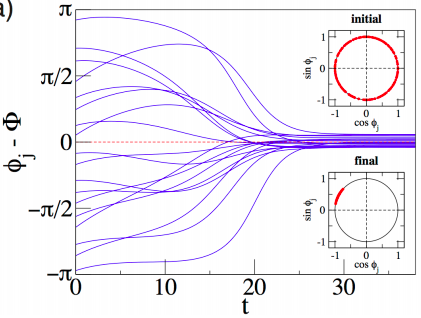
\includegraphics[width=0.45\textwidth]{kur100}
    \caption{
تحول زمانی فاز نوسانگرهای کوراموتو. در این شبیه‌سازی از ۱۰۰ نوسانگر استفاده شده است که فقط تحول زمانی فازهای ۱۸ عدد از نوسانگرها نمایش داده شده است. فرکانس ذاتی نوسانگرها به صورت تصادفی از توزیع نرمال (
$\mu=1.0$  و $\sigma=0.1$
) و فاز اولیه نوسانگرها نیز به صورت تصادفی از توزیع یکنواخت در بازه 
$[0,2\pi)$
انتخاب شده است. برای انتگرال‌گیری از روش اویلر با گام 
$dt\approx 0.01$
استفاده کرده‌ایم. واضح است که بعد از گذشت زمان همگامی نوسانگرها بیشتر شده است.
    }
%    \label{fig:dbs-protocols}
\end{figure}



\begin{figure}
	\centering
	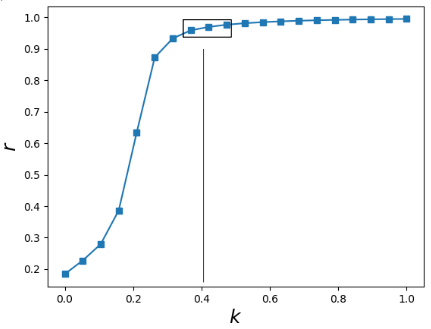
\includegraphics[width=0.45\textwidth]{kur1000orderParam}
    \caption{
نمودار اندازه پارامتر نظم بر حسب ضریب جفت شدگی. هر نقطه (برای هر مقدار ضریب جفت شدگی) از متوسط گیری پارامتر نظم ۴ سیستم با شرایط اولیه متفاوت تولید شده است. برای شبیه سازی هر سیستم از تعداد ۱۰۰۰ نوسانگر کوراموتو استفاده شده است. فرکانس ذاتی نوسانگرها به صورت تصادفی از توزیع نرمال (
$\mu=1.0$  و $\sigma=0.1$
) و فاز اولیه نوسانگرها نیز به صورت تصادفی از توزیع یکنواخت در بازه 
$[0,2\pi)$
انتخاب شده است. انتگرال‌گیری برای ۱۰۰۰ گام زمانی به طول
 $dt \approx 0.01$
 به روش اویلر انجام شده است که ۱۰ گام نهایی برای محاسبه پارامتر نظم آن سیستم میانگین گیری شده اند. محدوده مشخص شده در 
 $k \approx 0.4$
 محدوده مورد نطر ماست زیرا نوسانگرها به طور کامل همگام نمی‌شوند.
    }
    \label{fig:orderParam-k}
\end{figure}

اندازه پارامتر نظم معیاری از همگامی است؛ که مقادیر صفر و یک آن به ترتیب با حالت کاملا ناهمگام و حالت کاملا همگام متناظر هستند. وقتی تحریکی به سیستم وارد نشود، نوسانگرها تمایل به همگامی دارند. تمایل به همگامی توسط ضریب جفت شدگی کنترل می شود؛ به طوری که هرچه ضریب جفت شدگی بزرگ‌تر باشد همگامی سریع‌تر اتفاق میفتد. با توجه به اینکه ما در نظر داریم تحریک‌ را بر اساس فاز نوسانگرها اعمال کنیم، پس ضریب جفت شدگی را طوری انتخاب می‌کنیم که نوسانگرها کاملا همگام نشوند. بنابراین، با توجه به شکل 
\ref{fig:orderParam-k}
مقدار ضریب جفت‌شدگی 
$k \approx 0.4$
انتخاب می‌کنیم. در نهایت، بر اساس معادله تحول 
\ref{eq:kuramotoModelres}
در زمان‌های مختلف سیستم را تحریک می‌کنیم.

\begin{figure}
	\centering
	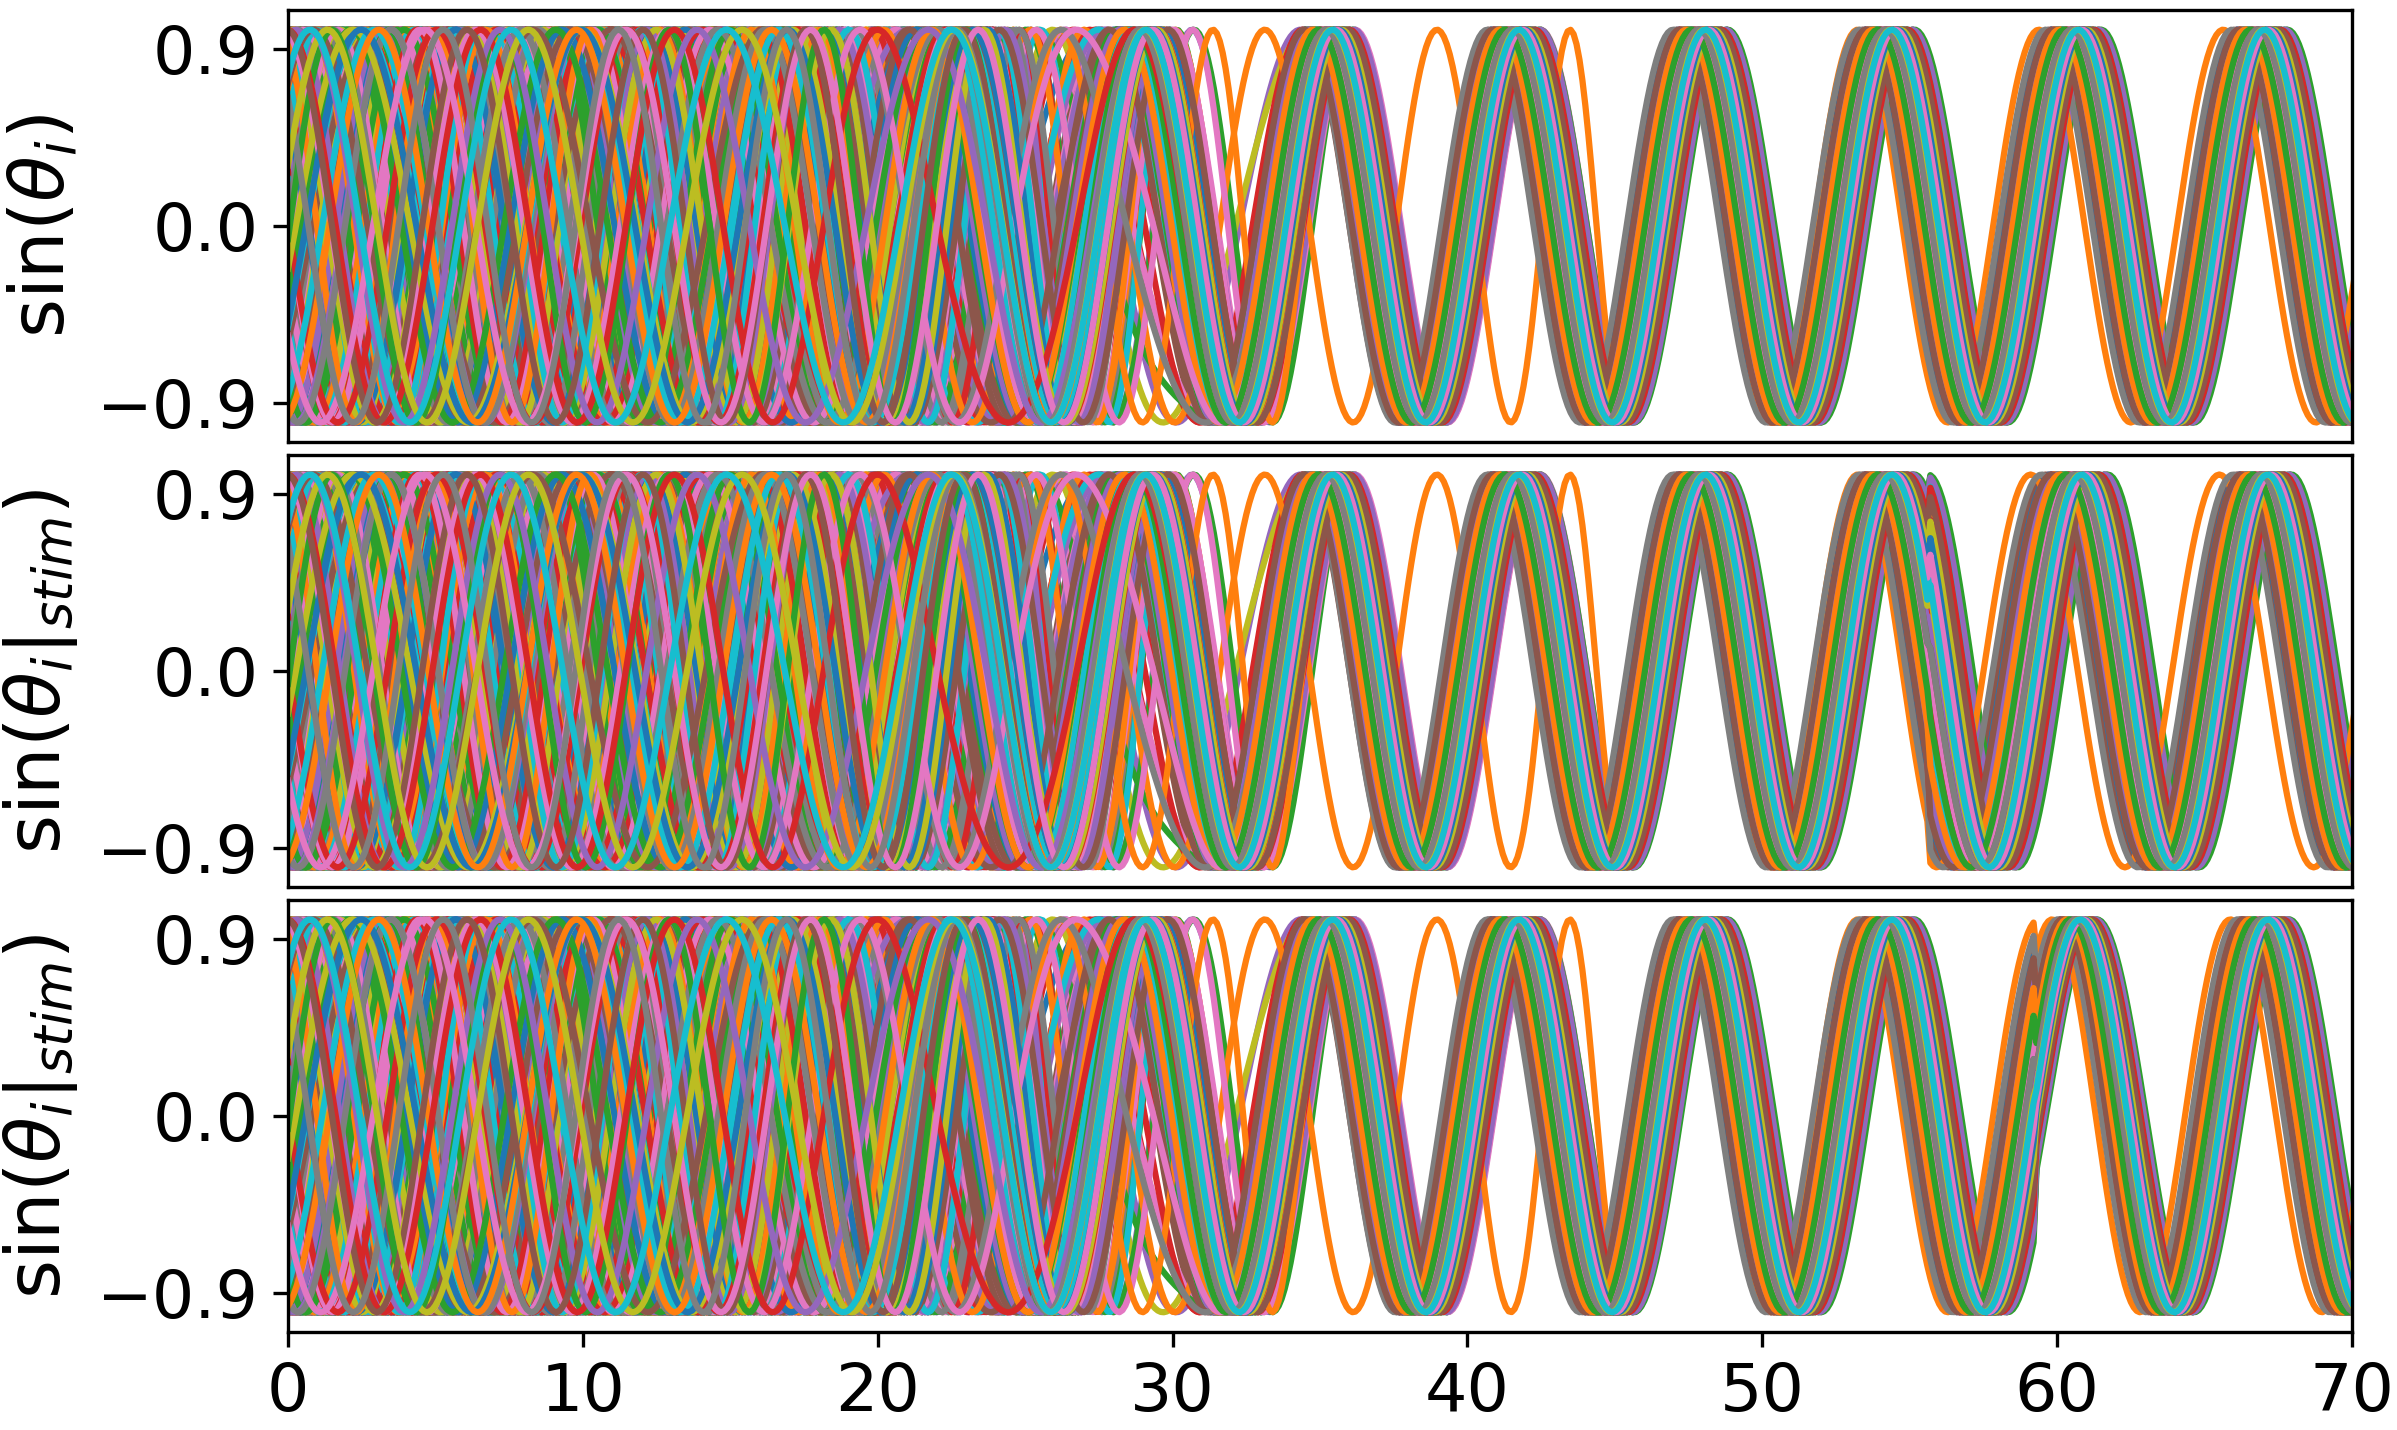
\includegraphics[width=0.9\textwidth]{kur1000-compare-thetas}
    \caption{
نمودار تحول فاز نوسانگرها در سه حالت مختلف. نمودار بالایی بدون اعمال تحریک. در نمودار میانی تحریک در لحظه 
$t=55.7$
و در نمودار پایینی در لحظه 
$t=59.3$
اعمال شده است.
    }
    \label{fig:kur-compare-thetas}
\end{figure}

در مورد شکل ها صحبت کن و دلتا ار رو معرفی کن.!!!!!!!!!!!!!!!!!!!!!!!!!!!!!!!!!!

\begin{figure}
     \centering
     \begin{subfigure}[t]{0.3\textwidth}
         \centering
         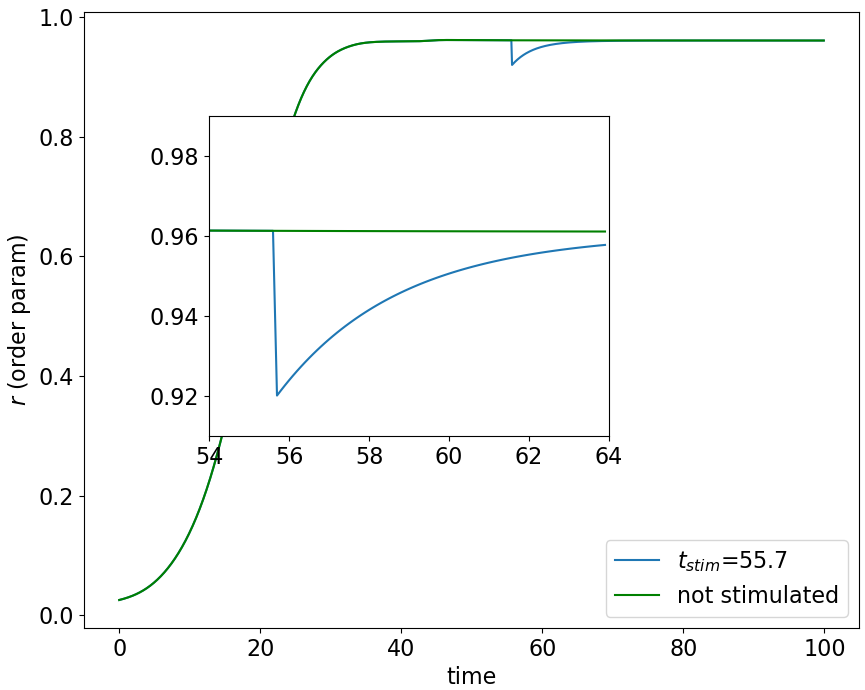
\includegraphics[width=\textwidth]{k1000stim-orderParam1}
%         \caption{الکترودهای تحریک عمیق مغز کاشته شده در سر }
%         \label{fig:tdcs}
     \end{subfigure}
     \
     %\hfill
     \begin{subfigure}[t]{0.2\textwidth}
         \centering
         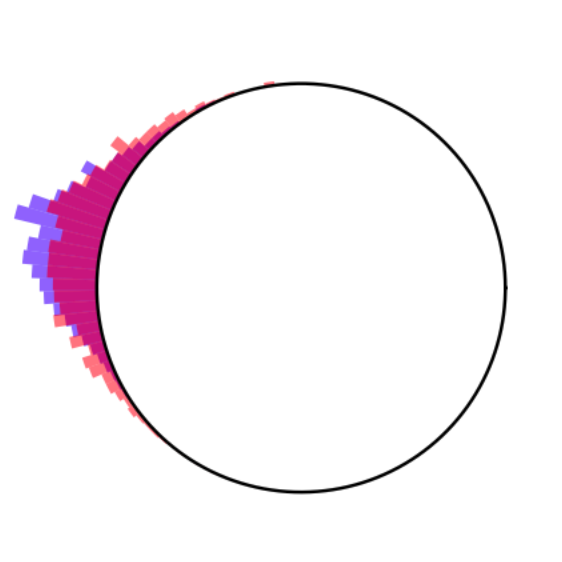
\includegraphics[width=\textwidth]{distro1}
%         \caption{الکترودهای تحریک عمیق مغز کاشته شده در سر }
%         \label{fig:tacs}
     \end{subfigure}
     \
  %   \hfill
     \begin{subfigure}[t]{0.4\textwidth}
         \centering
         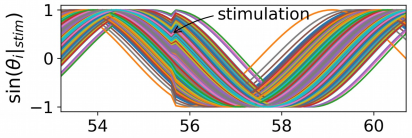
\includegraphics[width=\textwidth]{k1000theta-stim1}
%         \caption{    نوسان‌سازهای کار گذاشته شده درون قفسه سینه}
%         \label{fig:trns}
     \end{subfigure}
        \caption{
اعمال تحریک در لحظه 
$t=55.7$.
در شکل سمت چپ نمودار تحول زمانی فاز نوسانگرها را مشاهده می‌کنیم. در شکی میانی توزیع فاز در لحظه های قبل (آبی) و بعد (قرمز) از اعمال تحریک را می‌بینیم و در شکل سمت راست تحول زمانی پارامتر نظم برای سیستم تحریک شده (آبی) و سیستم تحریک نشده  (سبز).
         }
%        \label{fig:dbs-xray}
\end{figure}

\begin{figure}
     \centering
     \begin{subfigure}[t]{0.3\textwidth}
         \centering
         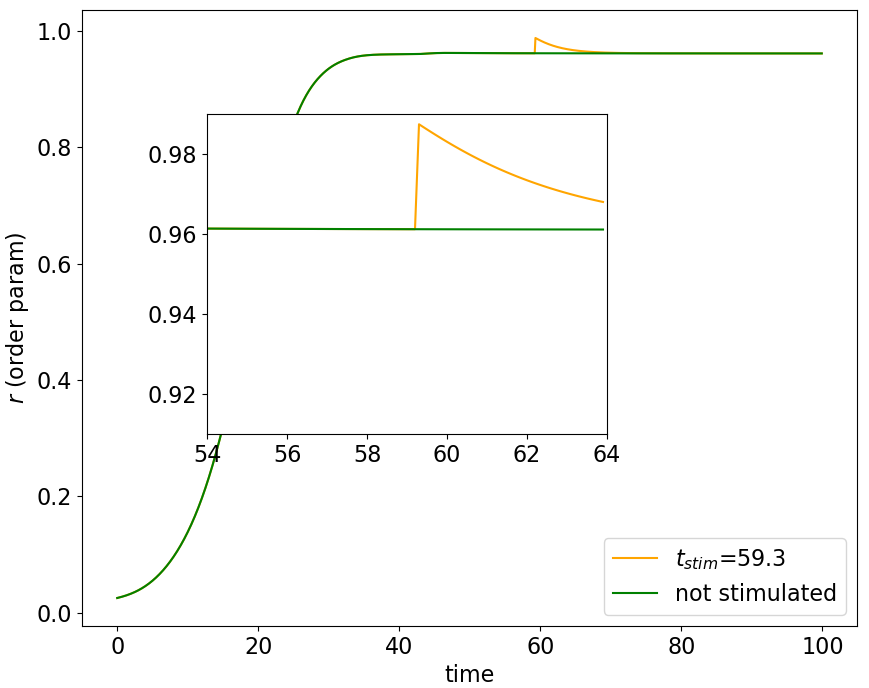
\includegraphics[width=\textwidth]{k1000stim-orderParam2}
%         \caption{ تحول زمانی پارامتر نظم }
%         \label{fig:tdcs}
     \end{subfigure}
     \
     %\hfill
     \begin{subfigure}[t]{0.2\textwidth}
         \centering
         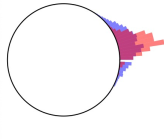
\includegraphics[width=\textwidth]{distro2}
%         \caption{فراوانی فاز نوسانگرها قبل و بعد از تحریک }
%         \label{fig:tacs}
     \end{subfigure}
     \
  %   \hfill
     \begin{subfigure}[t]{0.4\textwidth}
         \centering
         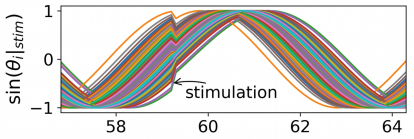
\includegraphics[width=\textwidth]{k1000theta-stim2}
%         \caption{تحول زمانی فاز نوسانگرها }
%         \label{fig:trns}
     \end{subfigure}
        \caption{
اعمال تحریک در لحظه 
$t=59.3$.
در شکل سمت چپ نمودار تحول زمانی فاز نوسانگرها را مشاهده می‌کنیم. در شکی میانی توزیع فاز در لحظه های قبل (آبی) و بعد (قرمز) از اعمال تحریک را می‌بینیم و در شکل سمت راست تحول زمانی پارامتر نظم برای سیستم تحریک شده (نارنجی) و سیستم تحریک نشده  (سبز).
         }
%        \label{fig:dbs-xray}
\end{figure}



\begin{figure}
	\centering
	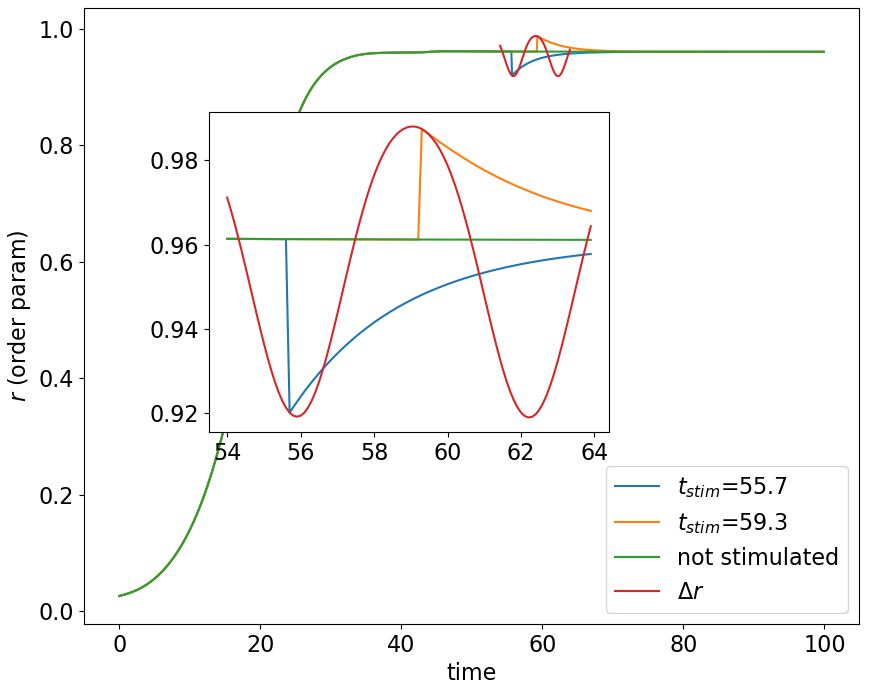
\includegraphics[width=0.5\textwidth]{k1000stim-orderParam}
    \caption{
بیشینه تغییرات پارامتر نظم سیستم تحریک شده و سیستم تحریک نشده بر حسب زمان اعمال تحریک.
    }
%    \label{fig:kur-compare-thetas}
\end{figure}




\begin{figure}
	\centering
	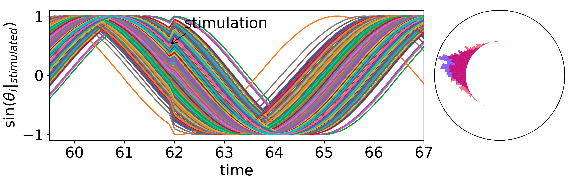
\includegraphics[width=0.7\textwidth]{theta-dist}
    \caption{
اعمال تحریک در لحظه 
$t=61.9$.
    }
%    \label{fig:kur-compare-thetas}
\end{figure}



\begin{figure}
	\centering
	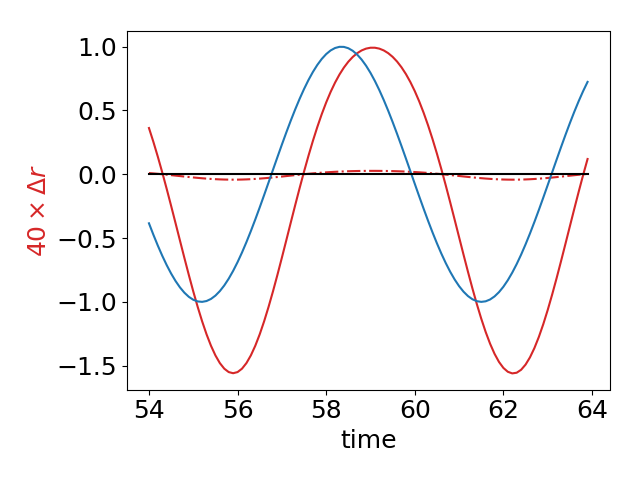
\includegraphics[width=0.6\textwidth]{orderParam-prc}
    \caption{
نمودار بیشینه تغییرات پارامتر نظم بین سیستم تحریک شده و تحریک نشده (خط نقطه قرمز) و تابع پاسخ فاز جمعیت (آبی).
    }
%    \label{fig:kur-compare-thetas}
\end{figure}

\begin{figure}
	\centering
	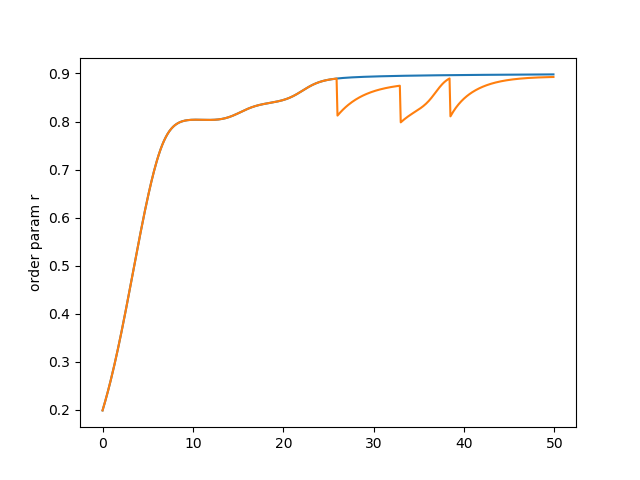
\includegraphics[width=0.6\textwidth]{multiple-stim}
    \caption{
با اعمال تحریک‌های پیاپی بر اساس فاز سیستم در دوره‌های مختلف می‌توان پارامتر نظم را کاهش داد و همچنین حالت دینامیکی سیستم را نیز تغییر داد.
    }
%    \label{fig:kur-compare-thetas}
\end{figure}

نوسانات همگام درون و بین نواحی مغز به پردازش عادی اطلاعات در مغز کمک می‌کنند؛ اما در برخی از بیماری‌های سیستم عصبی، این نوسانات در مقایسه با مغز سالم تقویت می‌شوند. به عنوان مثال می‌توان به نوسانات تقویت شده بتا (با فرکانس تقریبی ۲۰ هرتز) که بین قشر و هسته زیرتالاموسی در بیماران پارکینسونی ثبت شده است، اشاره کرد. تحریکِ عمیقِ مغز، درمانی مؤثر برای اختلالات عصبی متنوعی از جمله پارکینسون و لرزش اساسی است. در حال حاضر در روش تحریک عمیق مغز، قطاری از پالس‌های الکتریکی با بسامد ثابت توسط الکترود‌هایی که در مغز کاشته شده‌اند به محل‌های هدف در مغز اعمال می شوند.  تحریک عمیق مغز حلقه‌بسته یک رهیافت جدید و  امید‌بخش است که تحریک بر اساس وضعیت بیمار اعمال می‌شود. در این رهیافت جدید به جای آنکه از قطاری از پالس‌های با بسامد ثابت استفاده کنند، تحریک بر اساس فعالیت مغزی بیمار اعمال می‌شود.  این روش توانایی زیادی برای پیشرفت در بهره‌وری، ثمربخشی و کاهش اثرات جانبی دارد. بهبود این روش وابسته به ابداع کردن یک راهبرد تحریک است که نوسانات فعالیت‌های عصبی که نشانه بیماری هستند را کاهش دهد. یکی از راه‌های رسیدن به این هدف مدل سازی‌های نظری و محاسباتی است. این مدل سازی‌ها توصیف خوبی از نحوه تغییر نوسانات مغزی بعد از اعمال تحریک ارایه می‌دهند. برای مثال، مدل سازی های محاسباتی پیشنهاد می کنند که دامنه نوساناتی که نشانه بیماری هستند را می توان با اعمال تحریک در فازهای مشخصی از نوسانات، اصلاح کرد. در این مطالعه، در نواحی‌ای که نوسانات نشانه بیماری را تولید می‌کنند به جای نورون‌ها از نوسانگر های جفت شده استفاده می‌کنیم و نشان می دهیم که اگر در فاز و دامنه مشخصی تحریک را اعمال کنیم، سیستم عصبی چطور به آن تحریک پاسخ خواهد داد. همچنین نشان می‌دهیم که با توجه به منحنی پاسخ فاز نوسانگرها می‌توان بهترین زمان اعمال پالس را برای بیشترین کاهش در دامنه نوسان پیش‌بینی کرد.
%\section*{چرکنویس}
\subsection*{تحریک}




\underline{
این قسمت باید تحت عنوان تحریک مغز قرار بگیرد
}

تحریک مغز به عنوان یک درمان کمکی از اختلالات عصبی مختلف با موفقیت متغیر تحت تحقیق قرار گرفته است.

یک چالش ، دانش محدود در مورد اهداف عصبی موثر برای یک مداخله ، همراه با دانش محدود در مورد مکانیسم های عصبی تحریک مغز است.

از یک سو با انگیزه شواهد اخیر مبنی بر اینکه فعالیت های نوسانی در سیستم های عصبی در تنظیم عملکردها و اختلالات عملکرد مغز ، به ویژه موارد اختلالات عصبی ویژه بیماران مسن ، نقش دارند ،
و از طرف دیگر که ممکن است از تکنیک های تحریک مغز برای تعامل با این نوسانات مغزی به روشی کنترل شده استفاده شود ، ما در اینجا پتانسیل تعدیل نوسانات مغز را به عنوان یک استراتژی موثر برای مداخلات بالینی تحریک مغز بررسی می کنیم.

ما در ابتدا شواهد مربوط به پروفایل های نوسانی غیرطبیعی را که با طیف وسیعی از اختلالات عصبی در افراد مرتبط است (به عنوان مثال ، بیماری پارکینسون ، بیماری آلزایمر، سکته مغزی ، صرع) بررسی می کنیم.
سپس ، ما سیگنال های فعالیت غیر طبیعی شبکه را بررسی می کنیم تا با درمان نرمال شود و یا پیش بینی پیشرفت بیماری یا بهبودی آن باشد.
سپس این سوال را می پرسیم که پروتکل های  تحریک مغز موجود تا چه اندازه متناسب با این نوسانات و احتمالاً اختلالات عملکردی تنظیم شده اند.

با این حال ، تاکنون ، درک نقش این ریتم ها در رفتار انسان و بروز علائم در بیماری ها محدود است.


هزاران نورون فعالیت خود را همگام می کنند تا الگوی نوسانی نوعی تولید کنند که می تواند از طریق الکتروانسفالوگرام از الکترودهای روی پوست سر یا از طریق پتانسیل های میدان محلی  یا ضبط داخل جمجمه از الکترودهای کاشته شده در مغز اندازه گیری شود.

تکنیک های تحریک مغز با القای و تعدیل فعالیت نوسانی مداوم قادر به ایجاد تغییرات عملکردی در مغز هستند.بنابراین ، این تکنیک ها ممکن است نقش بالقوه ای در تشخیص و درمان اختلالات عصبی ، آشکار کردن پاسخ نوسانی غیرطبیعی و یا استفاده در تلاش برای برقراری تعادل مجدد فعالیت در مدارهای عصبی غیرطبیعی داشته باشند.


اتصالات درون مغز پویا هستند، که با افزایش سن تغییر می کند و می تواند با آموزش های شناختی و بدنی تعدیل شود.
گروههای مختلفی از سلولهای عصبی تمایل دارند که فعالیت خود را در فرکانسهای خاصی که به صورت ریتم تعریف شده اند همزمان کنند ، که در پنج باند فرکانسی طبقه بندی شده اند: دلتا (<4 هرتز) ، تتا (4-8 هرتز) ، آلفا (8-12 هرتز) ، بتا (12–30 هرتز) و گاما (30–90 هرتز). فرکانس های بالاتر (> 90 هرتز) به عنوان فعالیت نوسانی فرکانس بالا در نظر گرفته شده اند

\lr{ EEG} به راحتی می تواند نوسانات از باند دلتا تا بتا را تشخیص دهد ، در حالی که برای ضبط فعالیت های گاما و فعالیت نوسانی فرکانس بالا کمتر مناسب است ، زیرا شدت سیگنال این فعالیت ها در \lr{ EEG} از فعالیت فراوان (عمدتا عضله و جریان مستقیم اطراف) پوست سر خارج نمی شود.تأثیر محدود فعالیت عضلانی در \lr{MEG}و ضبط داخل جمجمه ، این دو روش را برای تحلیل نوسانات فرکانس بسیار بالا نیز مناسب می کند. در بخش های بعدی ، ما ادبیات موجود را به عنوان شواهدی در مورد نقش فیزیولوژیکی و پاتوفیزیولوژیکی این ریتم های مختلف بررسی خواهیم کرد.

شواهد متعددی نشان داده اند که فرکانس و یا فاز فعالیت نوسانی موضعی و همچنین فعالیت نوسانی بین نواحی مختلف از درگیری عملیات شناختی مختلف خبر می دهد که بر بروز رفتارهای خاص تاثیر میگذارند.
علاوه بر این ، نقایص عصبی مربوط به عملکردهای حرکتی ، دیداری-فضایی و حافظه با خرابی فعالیت نوسانی عصبی که در باندهای فرکانسی خاص در داخل و در سراسر نواحی مغز و قشر مغز فعالیت می کند ، مرتبط شده اند.

این گزارش ها علاقه مندی روزافزونی را برای دستکاری ریتم های مغزی انسان برای درک بهتر نقش علیت فیزیولوژیکی آنها در کدگذاری عملیات شناختی و درمان برخی از علائم اختلالات عصبی روانپزشکی همراه با اختلالات همزمان سازی عصبی ایجاد کرده است.

رویکردهای غیر تهاجمی تحریک مغزی ، مانند تحریک مغناطیسی یا تحریک جریان مستقیم، برای تقریباً دو دهه برای دستکاری و تعدیل فعالیت مغز استفاده شده است ، که نویدبخش نوعی درمان برای  بیماری های عصبی روانی است

اعمال این تکنیک ها با پارامترها و پیکربندی های تحریک مختلف (به عنوان مثال، تنظیم فرکانس یا فاصله بین برست های مختلف برای تحریک مغناطیسی) توانایی این را دارد تا تحریک پذیری سلول های عصبی را در محدوده مشخصی از مغز به صورت انلاین (همزمان) یا افلاین (طولانی مدت) تغییر دهد. همچنین این اثرات با دنبال کردن مسیر های اتصال درون مغز می تواند در میان شبکه های مغزی منتشر شوند. 


%\subsection{دلتا}
%در شرایط فیزیولوژیکی ، فعالیت دلتا برجسته ترین ویژگی  \lr{ EEG }در خواب حرکت غیر سریع چشم
%\LTRfootnote{ Non-rapid eye movement sleep (NREM) }
%انسان است.
%منشا آن نورونهای قشر مغز است و به عنوان یک واسطه احتمالی از انعطاف پذیری سیناپسی وابسته به خواب ارائه شده است که با همگام سازی حالت تحریک پذیری گروه های عظیمی از سلولهای عصبی قشر مغز فرایندهای حافظه کورتیکو-هیپوکامپ را تسهیل می کند.
%هنگام بیداری ، فعالیت دلتا در شرایط فیزیولوژیکی تقریباً وجود ندارد ،
%\\
%\lr{but it appears both after subcortical brain lesion sparing cerebral cortex and after the induction of cortical plasticity}

%\subsection{ الکتروانسفالوگرافی}
%نورون ها در شرایط خاصی تکانه الکتریکی کوچکی ایجاد می کنند؛ این تکانه ها اساس روش های ثبت الکتروفیزیولوژی هستند. گرچه هر نورون به تنهایی جریان خیلی کوچکی تولید می کند، قشر مغز از تعداد زیادی نورون تشکیل شده است؛ بنابراین اگر بسیاری از این نورون ها همزمان کار مشابهی انجام دهند، جریان های تولید شده به اندازه کافی بزرگ می شود، به طوری که از راه پوست سر می تواند ثبت گردد. این جریان ها باید بزرگ باشند؛ زیرا الکترودهای ثبت کننده روی پوست سر از منبع تکانه های الکتریکی با پرده های اطراف مغز، فضای مایع مغزی-نخایی، استخوان، چربی و پوست جدا شده است. به این ترتیب فعالیت ثبت شده در هر الکترود، به فعالیت کلی هزاران نورون وابسته است.
\subsection*{نوشته های جسته و گریخته که شاید درون متن بدرد بخوره}
ارتباطات نورونی وابسته است به مولفه های آناتومیک که نورون های منفرد را به هم وصل می کند (ساختاری) و فرآیند انتقال اطلاعات (عملکرد)؛ هر دو جنبه روی کارایی نهایی دستگاه عصبی اثر کی گذارند.


\lr{mean field models of neural populations under electrical stimulation-2020-plos computational biology:}

تحریک الکتریکی سیستم عصبی ابزاری کلیدی برای درک و مطالعه دینامیک شبکه های عصبی و در نهایت برای توسعه درمان بالینی است. بسیاری از کاربردهای تحریک الکتریکی جمعیت زیادی از سلول های عصبی را تحت تاثیر قرار می دهد و شبیه سازی و تحلیل شبکه های بزرگ نورونی کار سخت و دشواری است. ما در این مطالعه یک مدل تقلیل یافته میدان متوسط از نورون های مهاری و تحریکی 
\lr{AdExIF} 
را بررسی کرده ایم که می تواند در مطالعه اثرات تحریک الکتریکی روی جمعیت نورونی بزرگ استفاده شود. 

ورودی های الکتریکی ضعیف که به مغز در شرایط آزمایشگاهی (
\lr{in vivo} 
)
به کمک تحریک الکتریکی فراجمجمه ای یا در قشر جدا شده در شرایط آزمایشگاهی (
\lr{in vitro}
)
می تواند روی رفتار دینامیکی آن جمعیت نورونی تاثیر بگذارد. با این حال ساز و کارهای دقیقی که فعالیت کل جمعیت نورونی را کنترل و تنظیم می کند و اینکه چرا واکنش به تحریک در آزمایش ها بسیار متنوع هستند، هنوز به درستی درک نشده اند. علی رغم ناشناخته بودن جنبه های مختلف، تکنیک های تحریک الکتریکی برای درمان بیماری های عصبی در انسان ها در حال توسعه هستند. برای درک هر چه بهتر این برهمکنش ها، در بیشتر اوقات لازم است که شبکه بزرگی از نورون ها شبیه سازی و تحلیل شوند که از نظر محاسباتی بسیار دشوار است و نیاز به تلاش فراوان دارد. ما در این پژوهش یک مدل تقلیل یافته از جمعیت های نورونی جفت شده ارائه کرده ایم که نماینده تکه ای از بافت قشر مغز است. ما نشان دادیم که میدان های الکتریکی که اغلب در آزمایش های تحریک مغز بکار برده می شوند می تواند منجر به تقلید
\LTRfootnote{entrainment}
 نوسانات عصبی در سطح جمعیت شود.

اختلال وارد کردن به سامانه به منظور کشف خواص دینامیکی آن پارادایمی شناخته شده است که در علوم فیزیکی موفقیت آن ثابت شده است. این روش برای مقیاس های مختلفی که در سیستم عصبی مورد مطالعه قرار می گیرد نیز موفقیت های در خور توجهی داشته است. در مطالعات متعددی نشان داده شده است که روش های تحریک غیر تهاجمی مغز در شرایط آزمایشگاهی (
\lr{in vivo} 
)
مثل تحریک الکتریکی فراجمجمه ای با جریان متناوب (
\lr{tACS}
)
فعالیت نوسانی و همچنین عملکرد مغز را تغییر می دهد و روش های جدیدی را برای درمان اختلالات بالینی مثل صرع یا برای بهبود تثبیت حافظه در هنگام خواب فراهم کرده است. با این حال پژوهشگران هنوز به درک کاملی از چگونگی تاثیر تحریک الکتریکی بر شبکه های بزرگ نورونی دست نیافتند. به همین دلیل ما یک چارچوب محاسباتی برای مطالعه برهمکنش ورودی های الکتریکی متغیر با زمان با رفتارهای دینامیکی جمعیت های نورونی بزرگ ارایه کرده ایم.


\subsection*{چند سیناپسی با تاخیر}
این معادله معروف که معادله تحول ولتاژ غشا نورون هست، بدون تاخیر زمانی 
\begin{equation}
    \tau_m \frac{dv_i}{dt}=E_l-v_i-\sum_{j=1}^{N} r_m g_{ij}S_{ij}(v_i-E_{syn,j})
\end{equation}
این اندیس
$j$
در جمله 
$E_{syn,j}$
هم بخاطر این در نظر بگیریم که بعضی از نورون ها تحریکی و بعضی ها مهاری هستن که با وجود این اندیس
$j$
میشه بعدن شبکه ای درست کرد مخلوط از نورون های تحریکی و مهاری.

و این معادله که معادله تحول احتمال باز بودن  دریچه های یونی در سیناپس هست
\begin{equation}
    \tau_s \frac{dS_{ij}}{dt}=-S_{ij}
\end{equation}

\begin{figure}
    \centering
        \begin{tikzpicture}
        \Vertices{fig/tikzNet/3neuron1ver.csv}
        \Edges{fig/tikzNet/3neuron1edg.csv}
        \end{tikzpicture}
    \caption{نمای شبکه}
    \label{fig:3neuron1}
\end{figure}
برای مثال اگر قرار باشه همه معادلات مربوط به شبکه نشان داده شده در شکل 
\ref{fig:3neuron1}
را بنویسیم خواهیم داشت:


%\begin{equation}
    \begin{align}
        & \tau_m \frac{dv_1}{dt}=E_l-v_1 + R_m I_{ext} -r_m  g_{12}S_{12}(v_1-E_{syn,2}) -r_m  g_{13}S_{13}(v_1-E_{syn,3}) \\
        & \tau_m \frac{dv_2}{dt}=E_l-v_2+ R_m I_{ext} -r_m g_{21}S_{21}(v_2-E_{syn,1}) -r_m  g_{23}S_{23}(v_2-E_{syn,3}) \\
        & \tau_m \frac{dv_3}{dt}=E_l-v_3+ R_m I_{ext} -r_m g_{31}S_{31}(v_3-E_{syn,1}) -r_m  g_{32}S_{32}(v_3-E_{syn,2}) \\
        & \tau_s \frac{dS_{12}}{dt}=-S_{12} \\
        & \tau_s \frac{dS_{21}}{dt}=-S_{21} \\
        & \tau_s \frac{dS_{13}}{dt}=-S_{13} \\
        & \tau_s \frac{dS_{31}}{dt}=-S_{31} \\
        & \tau_s \frac{dS_{23}}{dt}=-S_{23} \\
        & \tau_s \frac{dS_{32}}{dt}=-S_{32} \\
    \end{align}
%\end{equation}

اگر قرار باشه تاخیر رو وارد کنیم معادله دیفرانسیل به شکل زیر تغییر می کنه
\begin{equation}
    \tau_m \frac{dv_i}{dt}=E_l-v_i-\sum_{j=1}^{N} r_m g_{ij}S{ij}(t-\tau_{ij})(v_i-E_{syn,j})
\end{equation}
اما معادله دوم(همان معادله تحول احتمال باز بودن دریچه های یونی در سیناپس) بدون تغییر باقی می مونه

\begin{figure}
    \centering
        \begin{tikzpicture}
        \Vertices{fig/tikzNet/2neurondelay1ver.csv}
        \Edges{fig/tikzNet/2neurondelay1edg.csv}
        \end{tikzpicture}
    \caption{نمای شبکه چند سیناپسی با تاخیر}
    \label{fig:2neurondelay1}
\end{figure}

برای مثال اگر قرار باشه معادلات مربوط به شبکه نشان داده شده در شکل 
\ref{fig:2neurondelay1}
را بنویسیم خواهیم داشت

\begin{equation}
    \begin{align*}
         \tau_m \frac{dv_1}{dt} & =E_l-v_1 + R_m I_{ext} \\
         \tau_m \frac{dv_2}{dt} & =E_l-v_2+ R_m I_{ext} -r_m g_{21}S_{21}(t-\tau_{21})(v_2-E_{syn,1}) \\ 
        & -r_m  g_{21'}S_{21'}(t-\tau_{21'})(v_2-E_{syn,1}) \\
         \tau_s \frac{dS_{21}}{dt} & =-S_{21} \\
    \end{align*}
\end{equation}


% \begin{figure}
%     \centering
%         \begin{tikzpicture}
%         \Vertex{A} \Vertex[x=2]{B}
%         \Edge[Direct](A)(B)
%         \end{tikzpicture}
%     \caption{کپشن}
%     \label{fig:my_label}
% \end{figure}

% \begin{figure}
%     \centering
%         \begin{tikzpicture}
%         \Vertices{vertices.csv}
%         \Edges{edges.csv}
%         \end{tikzpicture}
%     \caption{نمای شبکه}
%     \label{fig:my_label}
% \end{figure}


%------------------------------------------------

\begin{latin}
\bibliographystyle{unsrt}
\bibliography{ref}
\end{latin}

\end{document}